V rámci této práce bylo vytvořeno pět kooperujících nástrojů, které lze použít jak v textovém, tak grafickém režimu. Všechny nástroje jsou konfigurovatelné pomocí XML souborů či přímo v GUI. Veškeré nástroje byly implementovány v \texttt{C++} (standard \texttt{c++17}), pro grafickou nástavbu byl použit framework \texttt{Qt} verze $5$.

\section{Generátor produkčních dat}
Pro optimalizaci a vyhodnocení bylo nutno vytvořit generátor syntetických zákaznických objednávek. Není však možné, aby tyto generované objednávky byly čistě nahodilé, je třeba je generovat na základě nějakého matematického principu, a to z důvodu potřeby alespoň dvou sad objednávek, které budou různé ale budou spolu korelovat. První sada je použita pro optimalizaci skladu (dále nazývaná jako trénovací sada) a druhá pro vyhodnocení kvality optimalizace (dále nazývána jako testovací sada). Myšlenka je taková, že se vyhodnotí simulace skladu na testovací sadě objednávek a uloží se simulovaná doba. Poté se provede optimalizace na trénovací sadě objednávek a na tomto optimalizovaném modelu skladu se opět provede simulace na testovací sadě objednávek. Poté se porovná výsledná doba obou běhů simulace (před a po optimalizaci).

\begin{figure}[t]
    \centering
    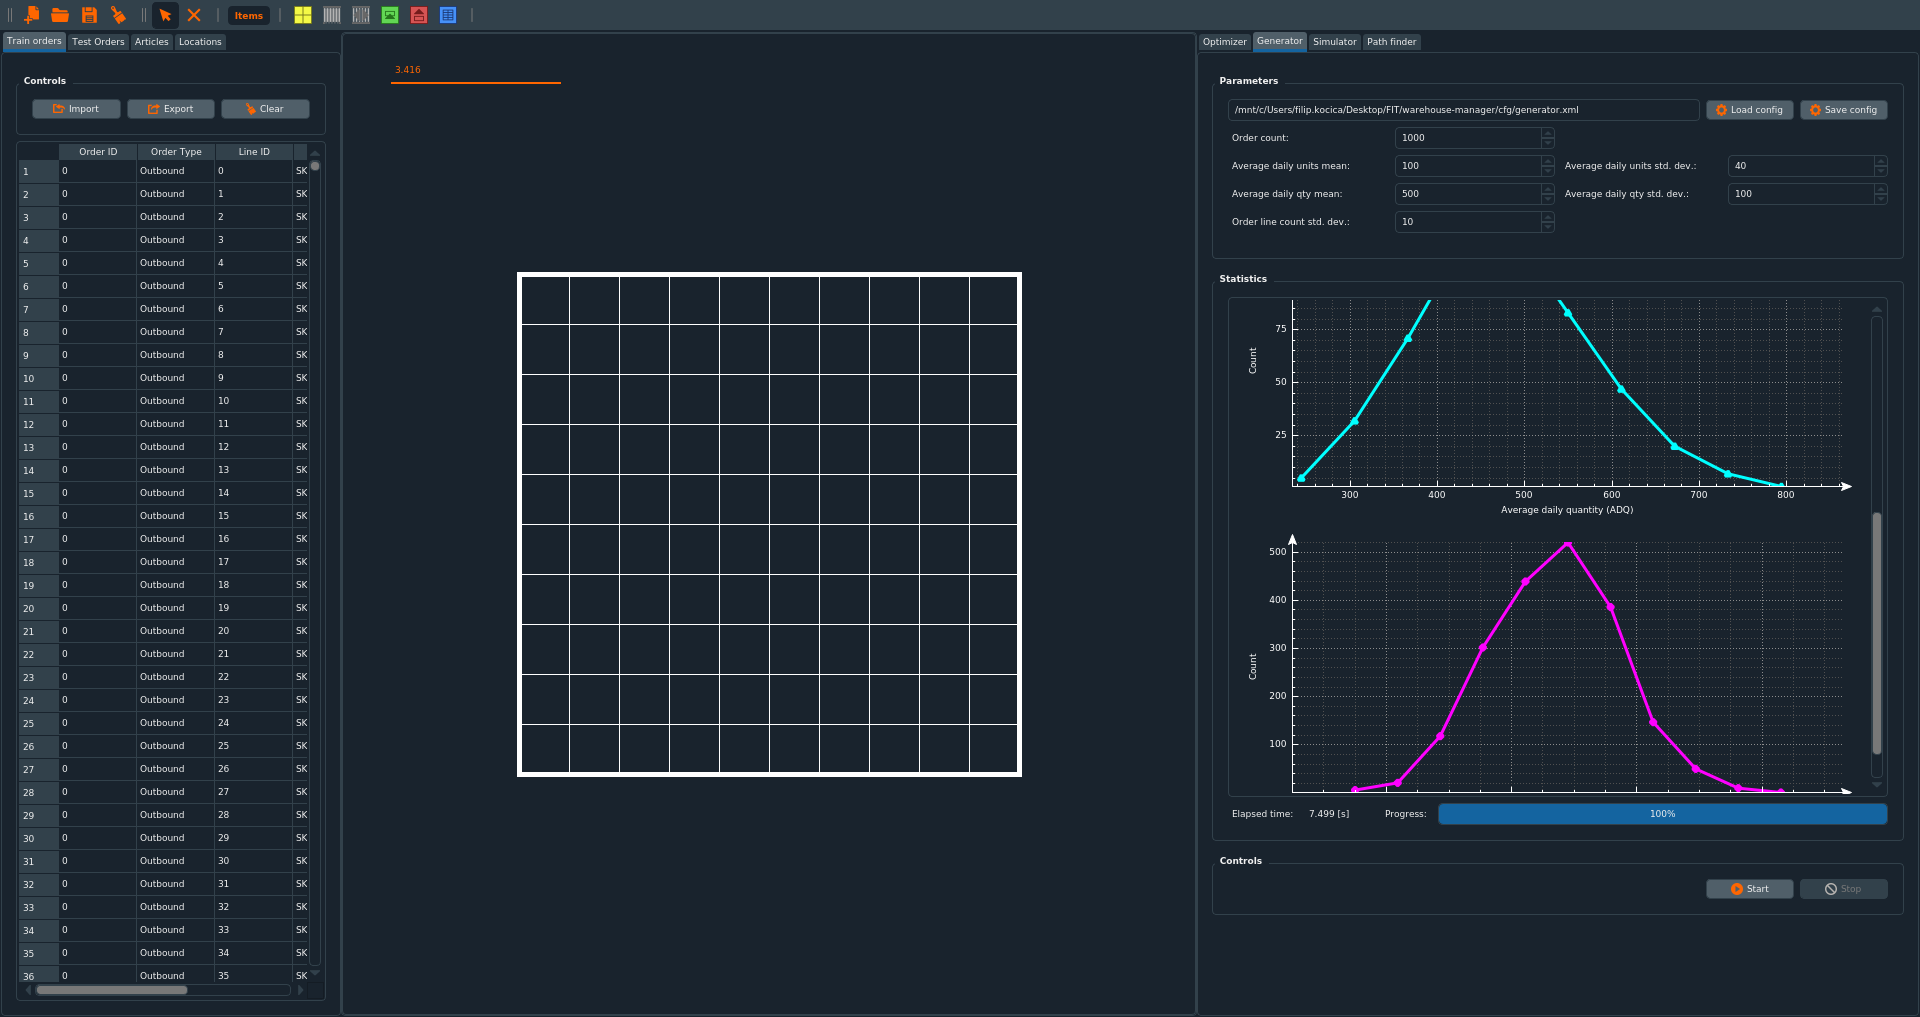
\includegraphics[width=0.99\linewidth]{figures/implementace/WarehouseManagerGen.png}
    \caption{Grafická implementace generátoru objednávek zakomponovaná do aplikace Warehouse Manager. Uprostřed je plocha pro tvorbu modelu skladu. Vpravo je kontrolní panel, kde je možné načíst a nastavit veškeré parametry generování, sledovat tři grafy normálních rozložení (vytvořených z generovaných dat) a spustit či zastavit generování. Vygenerovaná data jsou uložena do panelu s daty vlevo, kde je lze použít pro optimalizátor (první záložka s trénovacími daty), pro simulátor a pathfinder (druhá záložka s testovacími daty), nebo je možné tyto objednávky serializované exportovat do souboru na disk a~opětovně je poté načíst.}
    \label{fig:UI_generator}
\end{figure}

\subsection{Konfigurace}
Generátor objednávek, stejně jako ostatní nástroje, je závislý na vstupu od uživatele, a~proto bylo nutné implementovat způsob zadávání potřebných hodnot. K tomu byly využity konfigurační soubory ve formátu XML. Při použití grafického rozhraní je možné nastavit všechny parametry přímo tam, jak lze vidět na snímku \ref{fig:UI_generator}.

Jednotlivé položky které je uživatel schopen nastavit a jejich významy jsou následující (podrobnější vysvětlení lze najít v sekci \ref{section:impl_gen}):

\begin{itemize}
    \item \texttt{orderCount} -- Počet generovaných objednávek.
    \item \texttt{miAdu} -- Střední hodnota normálního rozložení pro generování ADU produktů.
    \item \texttt{sigmaAdu} -- Rozptyl normálního rozložení pro generování ADU produktů.
    \item \texttt{miAdq} -- Střední hodnota normálního rozložení pro generování ADQ produktů.
    \item \texttt{sigmaAdq} -- Rozptyl normálního rozložení pro generování ADQ produktů.
    \item \texttt{sigmaLines} -- Rozptyl počtu položek objednávek.
\end{itemize}

\subsection{Princip fungování a implementace}
\label{section:impl_gen}
Parametry generovaných sad objednávek, což jsou jejich množství, obsah a velikost, jsou dány uživatelem definovanými pravděpodobnostními rozděleními. Pravděpodobnostní modely, na základě kterých se generování provádí, jsou Gaussova rozložení -- parametry (střední hodnotu a rozptyl) definuje uživatel. Generátor je založen na hodnotách ADU\footnote{\emph{Average daily units} -- průměrný denní počet zakoupení.} a ADQ\footnote{\emph{Average daily quantity} -- průměrná denní zakoupená kvantita.}.

Samotné generování probíhá tak, že se vygeneruje hodnota ADU pro každý produkt $i$~a~spočtou se pravděpodobnosti zakoupení jednotlivých produktů $p_i$ pomocí rovnice:
\begin{equation}
    \label{eq:aduPst}
    p_i = \frac{ADU_i}{\sum_{n=1}^{N} ADU_n},
\end{equation}
z čehož vznikne diskrétní pravděpodobnostní rozložení. Poté se iteruje přes počet objednávek, které chce uživatel vygenerovat. Pro každou takovou objednávku se z normálního rozložení vygeneruje počet položek, které má tato objednávka mít. Poté je pro každou položku nutno vybrat produkt. To se provádí náhodným výběrem z pravděpodobnostního rozložení z rovnice \ref{eq:aduPst}, a tedy čím větší má produkt spočtenou pravděpodobnost zakoupení, tím má vyšší šanci výběru do objednávky. Nakonec se projdou všechny objednávky i jejich položky a pro každou z položek je vygenerována kvantita (zakoupené množství). To se provede tak, že vygenerovaná hodnota z rozložení ADQ pro daný produkt se vydělí počtem zakoupení tohoto produktu, tedy vygenerovaná kvantita se rozdělí mezi zakoupené produkty.

To ve výsledku dává tři Gaussova rozložení, první pro ADU, druhé pro ADQ a třetí pro počet položek objednávky. Vzhledem k tomu, že obě sady objednávek jsou generovány ze stejných pravděpodobnostních rozložení, vzniklé sady jsou různé, avšak spolu korelují.


\section{Simulátor skladu}
Účelem tohoto nástroje je odsimulování zpracování importovaných či generovaných objednávek na vytvořeném modelu skladu tak, jako by to byl reálný skladový systém. Lze jej použít samostatně (např. pro identifikaci úzkých míst, či pro statistickou analýzu), avšak jeho hlavní účel je aproximace kvality nalezeného řešení v optimalizátoru rozložení produktů~--~jinými slovy je použit jako objektivní funkce. Grafickou reprezentaci simulátoru lze vidět na snímku \ref{fig:UI_simulator}.

Autoři práce~\cite{whModelSim} zmiňují, že ze všech možných druhů je nejvhodnější a nejpřirozenější simulace skladu pomocí diskrétních událostí, protože sklad je v podstatě kolekce entit, které reagují na fixní diskrétní události. Simulátor je tedy založen na principu diskrétní simulace a při implementaci byla využita knihovna \texttt{SIMLIB/C++}\footnote{\emph{Simulation Library for \texttt{C++}} -- \url{http://www.fit.vutbr.cz/~peringer/SIMLIB}}. Simulátor poskytuje poměrně komplexní konfiguraci, což umožňuje rozsáhlé možnosti experimentování (od nastavení rychlostí pracovníků a dopravníků až po doplňování produktů, viz \ref{replenishment}).

\subsection{Konfigurace}
Stejně jako předchozí nástroj, je i simulátor konfigurovatelný, a to buď přímo v grafickém rozhraní, nebo \texttt{XML} souborem při použití textového rozhraní. Jednotlivé položky, které je uživatel schopen nastavit a jejich významy jsou následující:

\begin{itemize}
    \item \texttt{toteSpeed} -- Tato hodnota udává, jak rychle jezdí kartony po dopravnících a udává se v metrech za sekundu.
    \item \texttt{workerSpeed} -- Udává rychlost pracovníka, to znamená jak rychle se dokáže pohybovat a vytahovat produkty ze slotů lokací. Opět v metrech za sekundu.
    \item \texttt{totesPerMin} -- Udává, kolik kartonů/objednávek dokáže sklad odeslat za jednu minutu.
    \item \texttt{simSpeedup} -- Umožňuje zrychlení či zpomalení simulace.
    \item \texttt{locationCapacity} -- Udává, kolik objednávek je možné zároveň zpracovávat na jedné lokaci (lze chápat jako počet pracovníků na lokaci).
    \item \texttt{conveyorCapacity} -- Udává, kolik kartonů je možné zároveň převážet pomocí jednoho dopravníku.
    \item \texttt{orderRequestInterval} -- Udává interval, po jehož uplynutí přichází do systému nová objednávka.
    \item \texttt{replenishment} -- Udává, zda má systém počítat s kvantitami produktů a tedy s jejich doplňováním v případě nutnosti.
    \item \texttt{initialSlotQty} -- Tato hodnota říká, jaká je počáteční kvantita produktů v jednotlivých slotech.
    \item \texttt{replenishmentQuantity} -- Udává, kolik produktů se bude doplňovat.
    \item \texttt{replenishmentThreshold} -- Pokud počet produktů ve slotu klesne pod tuto hodnotu, je pro daný produkt spuštěno doplňování produktů.
    \item \texttt{preprocessing} -- Před-zpracování objednávek aby se zrychlila/zjednodušila simulace (tzn. seřazení položek objednávky, aby cesta skladem byla kratší):
    \begin{itemize}
        \item \texttt{None} -- Žádné předzpracování.
        \item \texttt{Normal} -- Předzpracování založené na jednoduchém pravidle porovnávající Manhattanské vzdálenosti jednotlivých lokací. 
        \item \texttt{Optimized} -- Pro každou objednávku je nalezena optimální cesta skladem pomocí nástroje pathfinder, popsaného v sekci \ref{sec:pathFinder}.
    \end{itemize}
\end{itemize}

\begin{figure}[t]
    \centering
    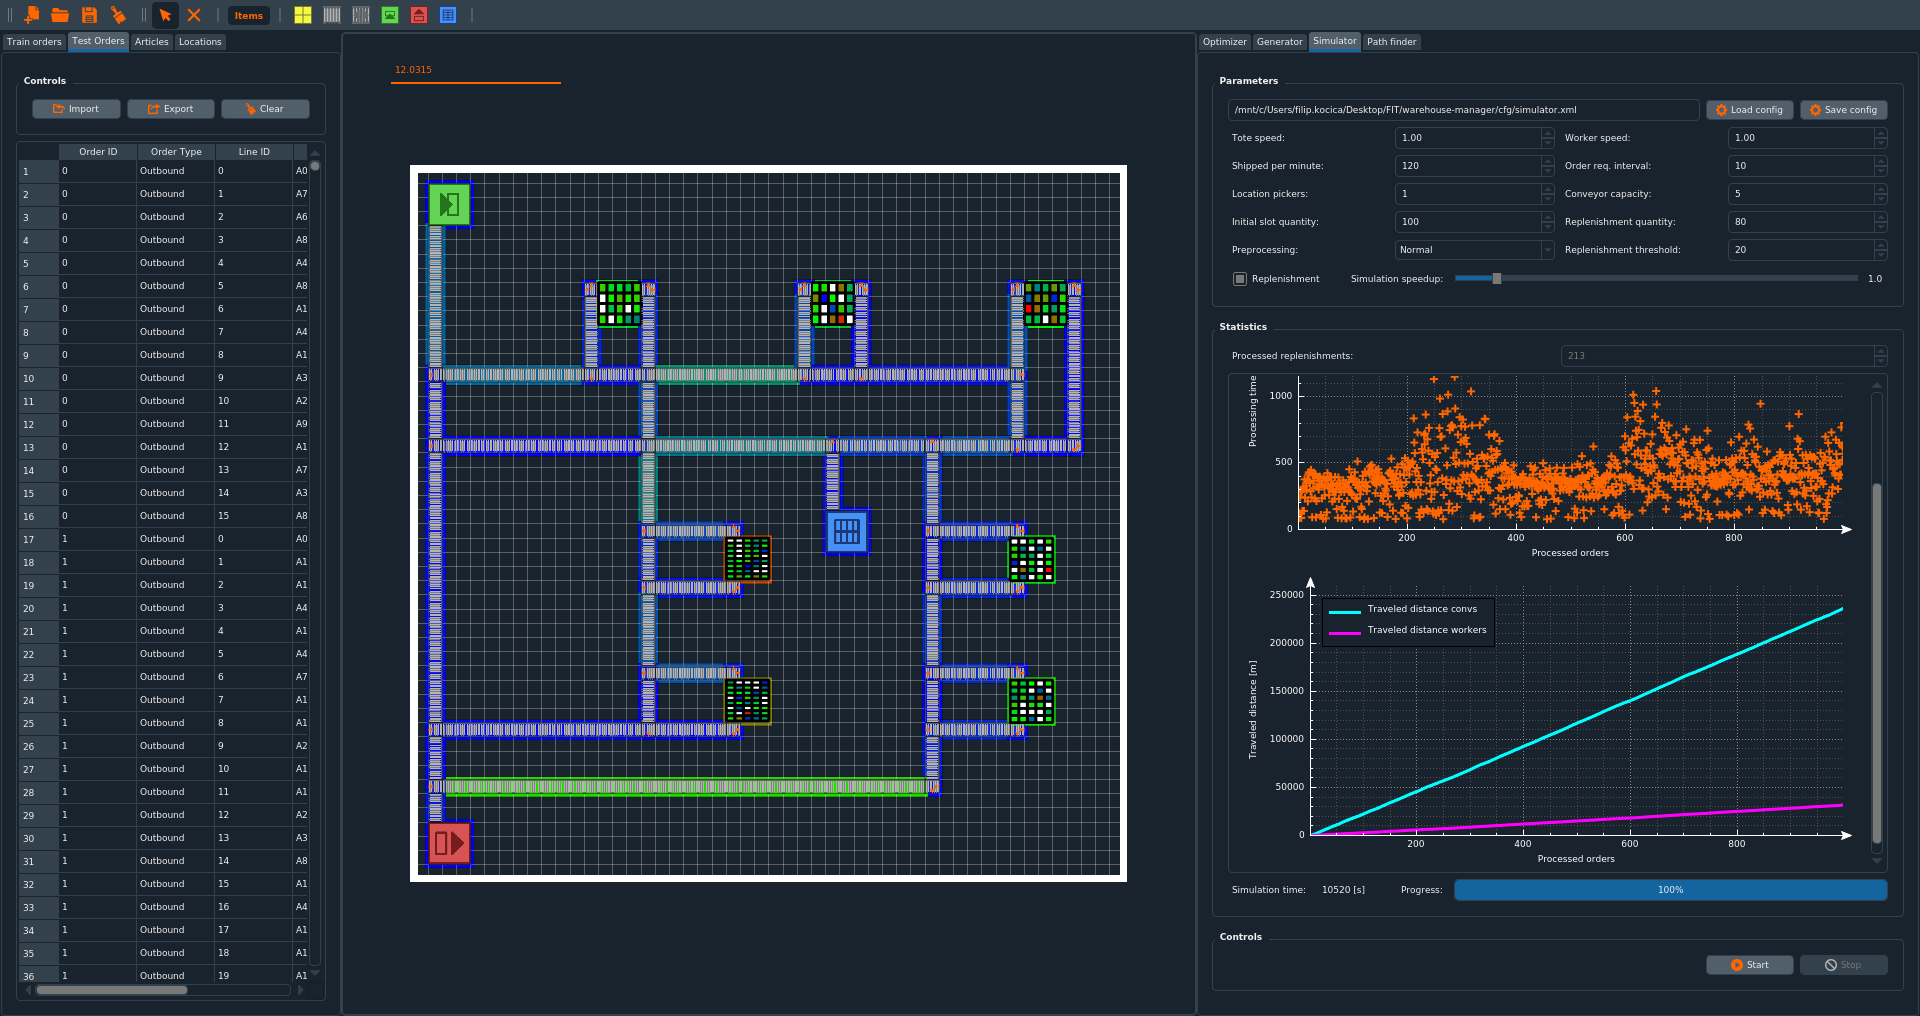
\includegraphics[width=0.99\linewidth]{figures/implementace/WarehouseManagerSim.png}
    \caption{Grafická implementace simulátoru skladu zakomponovaná do aplikace Warehouse Manager. Uprostřed je stále plocha pro tvorbu modelu skladu. Vpravo je kontrolní panel, kde je možné nastavit parametry simulace, sledovat grafy simulace (časy dokončení jednotlivých zákaznických objednávek, nárůst ujeté vzdálenosti na dopravnících a ušlé vzdálenosti pracovníků), vidět počet dokončených doplňovacích objednávek a kontrolovat simulaci (spustit, zastavit). Vlevo jsou data, které simulátor používá, jako je testovací sada objednávek a alokace produktů do slotů lokací. V modelu skladu lze vidět, které sloty lokací jsou zaplněny a je zobrazena také teplotní mapa produktů v lokacích i jednotlivých grafických prvků, kterou lze vidět na snímku~\ref{fig:heatmap} a která reprezentuje zatížení prvků.}
    \label{fig:UI_simulator}
\end{figure}

\subsection{Princip fungování a implementace}
Na začátku se provede načtení objednávek, modelu skladu a alokace produktů do slotů lokací. Poté se provede před-počítání všech možných cest ve skladu, jejich ohodnocení (délka v metrech) a seřazení od nejvýhodnější po nejméně výhodnou. Tímto způsobem lze získat nejvýhodnější cesty mezi všemi prvky/zařízeními ve skladu. Způsob zpracování je popsán pomocí PT sítě na snímku \ref{fig:PTsim}.

%Objednávky jsou modelovány jako diskrétní události (\texttt{class OrderRequest\_t : public simlib3::Event}), které do systému přichází v konfigurovatelných intervalech daných exponenciálním rozložením. Takováto diskrétní událost invokuje zpracování příchozí objednávky pomocí diskrétního procesu \texttt{class OrderProcessor\_t : public simlib3::Process}. Poté se prochází jednotlivé položky objednávky a pro každou z nich se provede vyhledání produktu ve skladu. Po jeho nalezení je nalezena (před-počítaná) optimální cesta a karton se vydává na cestu k cílové lokaci. Přitom projíždí přes jednotlivé dopravníky, které si alokuje pomocí volání knihovny \texttt{SIMLIB}, a sice \texttt{void Enter(Store &s, unsigned long ReqCap=1);}. Výpočet doby, po kterou přes daný dopravník má karton jet se provádí na základě zadaných parametrů, délky dopravníku a velikosti kartonu. Následuje uspání procesu na tuto vypočtenou dobu pomocí volání \texttt{virtual void Wait(double dtime);}. Po probuzení je kapacita opět uvolněna pro následující kartony pomocí volání \texttt{void Leave(Store &s, unsigned long ReqCap=1);}. Tímto způsobem \uv{dojede} karton po jednotlivých dopravnících až k cílové lokaci, ve které se nachází požadovaný produkt. Daný proces si opět alokuje zařízení, v tomto případě lokaci (tzn. další příchozí kartony modelované jako procesy musí čekat, než proces alokující lokaci dokončí práci). Až přijde karton na řadu, tak se opět uspí na vypočtenou dobu, čímž se simuluje pickování pracovníkem skladu nebo robotem. Tato doba je opět dána umístěním produktu v lokaci a nastavenými parametry. Po probuzení a navrácení kapacity se pokračuje další položkou v objednávce a pokračuje se stejným principem. Poté, co jsou všechny položky objednávky zpracovány, karton míří do oblasti odesílání (ang. \emph{shipping area}). Ze zadaných parametrů je vypočtena doba odesílání a je alokována odesílací rampa, proces je uspán a po uplynutí vypočtené doby opět uvolněna kapacita, a tím je objednávka považována za vyřízenou a zahrnuta do statistik. Po zpracování poslední objednávky je uložena nejdůležitější výstupní hodnota, a sice doba která je potřebná ke zpracování všech zadaných objednávek, v daném layoutu skladu a zejména \textbf{s danou alokací produktů do slotů lokací}.

\begin{figure*}[t]
    \centering
    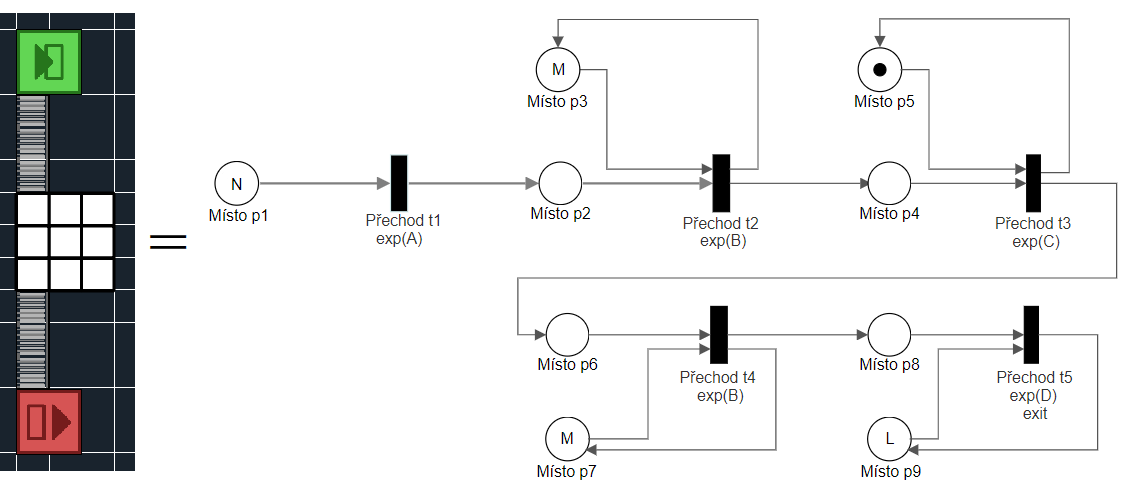
\includegraphics[width=0.71\linewidth]{figures/implementace/PT_wh.png}
    \caption{Triviální sklad se vstupem, jednou lokací a výstupem propojených dopravníkem. Vpravo je odpovídající PT síť. Na začátku se nachází místo \texttt{p1} s \texttt{N} tokeny, kde \texttt{N} se rovná počtu objednávek, které chceme ve skladu zpracovat. Tyto objednávky přichází do systému v časových intervalech (\texttt{A}) daných exponenciálním rozložením. Po vstupu objednávky musí její karton vjet na dopravník. Ten má však omezenou kapacitu danou výpočtem délka dopravníku děleno velikost jednoho kartonu (\texttt{M}). Doba po kterou jede karton po dopravníku je vypočtena jako poměr délky dopravníku a rychlosti kartonu (\texttt{B}). Poté karton vjede do lokace, kde si alokuje pickera na dobu (\texttt{C}), která je spočtena jako suma doby pickování všech produktů, které se v této lokaci mají pickovat. Obdobně karton projede další dopravník a nakonec je karton odeslán ze skladu -- je spočtena doba odesílání jedné objednávky (\texttt{D}), a také kolik jich lze odesílat zároveň (\texttt{L}). Vesměs všechny hodnoty v celém procesu jsou konfigurovatelné.}
    \label{fig:PTsim}
\end{figure*}

\subsection{Paralelní simulace}
\label{section:sim_multithreaded}
Simulátor je využíván mj. optimalizačním nástrojem pro vyhodnocení kvality řešení. Taková simulace je spouštěna pro každého jedince populace v každém kroku evolučního algoritmu. To v případě velkých populací vede k velmi dlouhému trvání optimalizace. Vzhledem k~tomu, že knihovna \texttt{SIMLIB/C++} nebyla koncepčně navržena pro účely paralelního zpracování, nebylo možné provést zrychlení použitím více vláken.

\begin{figure*}[t]
    \centering
    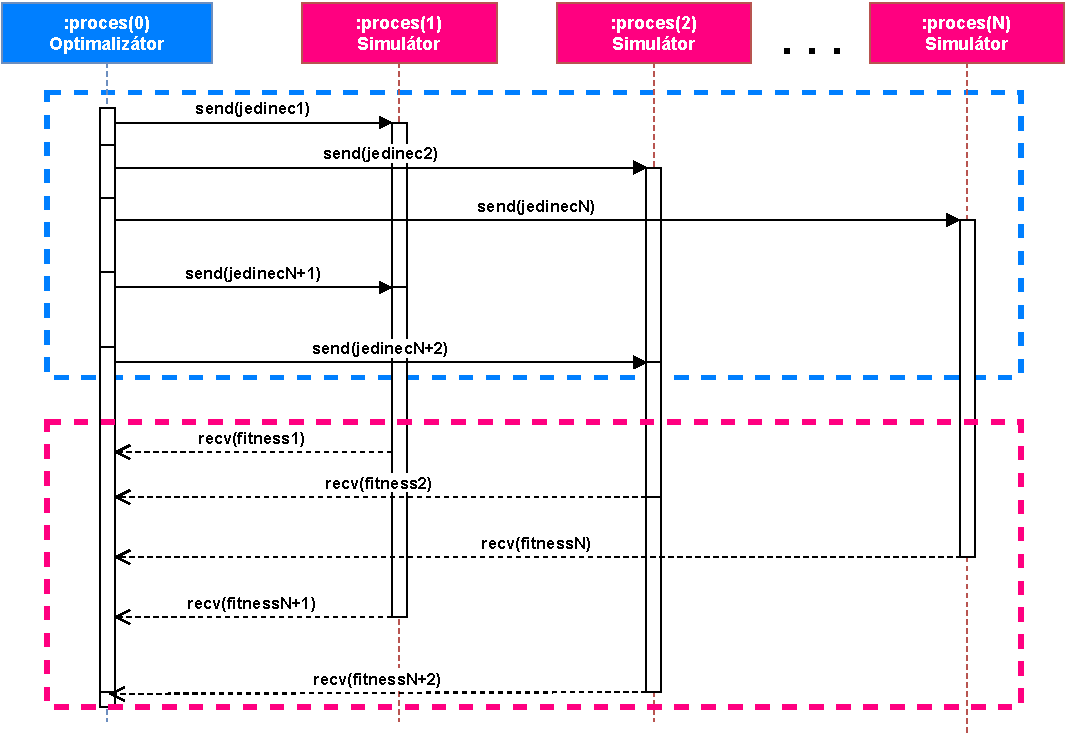
\includegraphics[width=0.8\linewidth]{figures/implementace/SimulationMessageSequence.pdf}
    \caption{Sekvenční diagram znázorňující paralelizaci optimalizace (rovnoměrné rozdělení výpočtu simulací všech jedinců populace mezi $N$ procesů). Modrý obdélník označuje odeslání jedinců na simulaci a růžový pak vysbírání výsledků doby simulace od jednotlivých potomků.}
    \label{fig:simulationMsgSeq}
\end{figure*}

Tento problém byl vyřešen spuštěním několika instancí (procesů) využívající tuto knihovnu, které se nijak neovlivňují a mohou fungovat souběžně. Před začátkem optimalizace je tedy vytvořeno $N$ (konfigurovatelné) takových procesů. Účel takto vytvořených potomků je jednoduchý, a sice provést inicializaci (objednávek, modelu skladu a před-počítání cest), očekávat data, provést simulaci a vrátit výsledek simulace hlavnímu procesu. Po odeslání dat zpět rodiči potomek opět vstupuje do blokujícího čekání na data nebo ukončení komunikace a tedy i samotného potomka. Komunikace mezi rodičem a potomky je znázorněna na snímku~\ref{fig:simulationMsgSeq}.

\begin{itemize}
    \item Od rodiče k potomkům se posílá zakódovaná alokace produktů do jednotlivých slotů (celočíselné pole).
    \item Od potomků zpět k rodiči se posílá výsledek (doba) simulace, a sice hodnota \emph{fitness} (číslo s plovoucí řádovou čárkou).
\end{itemize}

Jedinci (potažmo jejich simulace) jsou mezi procesy rozděleny zcela rovnoměrně a zrychlení optimalizace pomocí paralelizace simulací bylo velmi značné.



\subsection{Řešení problému duplicitních jedinců}
\label{section:sim_duplicit_jedinci}
Dále bylo zjištěno, že až $30\%$ všech jedinců v populaci je duplicitních (stejných jako nějaký jiný jedinec). Byl proto implementován mechanismus převodu zakódovaných genů jedince na řetězec, a pomocí hashovací tabulky bylo zajištěno, že se nebudou provádět duplicitní simulace, ale jedinci se stejnými geny si pouze překopírují již spočtený výsledek jiného jedince. To vedlo k ještě většímu zrychlení celého procesu a optimalizace i opravdu komplexního skladu bylo možné počítat v řádu maximálně několika dní.

\subsection{Doplňování produktů}
\label{replenishment}
%Doplňování produktů (ang. \emph{replenishment}) je proces, při kterém se ze zásobníku produktů (označován jako \emph{buffer}) doplňují produkty do slotů lokací, ze kterých se následně pickují zákaznické objednávky. Toto se typicky provádí ve chvíli, kdy množství produktů ve slotu klesne pod určitou úroveň (konfigurovatelná v XML/UI). Tento mechanismus byl implementován za účelem zvýšení realističnosti simulace skladu.

%Implementace doplňování produktů je následující: do konfigurátoru skladu byl přidán nový grafický prvek, zásobník produktů, ze kterého se budou produkty doplňovat do lokací a uživatel si jej může umístit kam chce (a připojit dopravníkem ke zbytku skladu). Následně byl přidán nový typ objednávky, a tedy se v systému mohou vyskytovat dva typy objednávek:

%\begin{enumerate}
%    \item \emph{Outbound} -- odchozí zákaznická objednávka.
%    \item \emph{Replenishment} -- interní objednávka určená pro doplňování produktů.
%\end{enumerate}

%Objednávka pro doplňování je v podstatě úplně stejná jako odchozí zákaznická objednávka, liší se pouze typem. Je tedy také zpracovávána pomocí diskrétního procesu \texttt{class OrderProcessor\_t : public simlib3::Process}. V případě, že v některé z lokací klesne množství produktů ve slotu pod konfigurovanou úroveň, je vytvořena objednávka pro doplňování a jsou ji přidány položky se všemi produkty, které jsou v dané lokaci a jejich kvantita je pod danou úrovní. Kvantita položek je nastavena na předem konfigurovanou hodnotu. Tato objednávka je stejně jako odchozí objednávka reprezentována jako proces v systému a po cestě ze zásobníku k lokaci se chová úplně stejně. Poté, co se objednávka pro doplnění dostane do cílové lokace, jsou veškeré produkty z objednávky doplněny do slotů lokace, kam patří (což pracovníkovi opět zabere jistý čas podle pozice slotu).

%\paragraph{Objednávky, které nelze napickovat} Může se stát, že množství produktů ve slotu klesne pod kvantitu, kterou vyžaduje některá z odchozích objednávek. Takovou objednávku nelze v daný moment dokončit a proces dané objednávky je deaktivován a musí čekat na doplňovací objednávku, což lze v systému chápat jako penalizaci. Poté, co přijde objednávka pro doplnění produktů a je dokončena, jsou všechny takto deaktivované procesy reprezentující odchozí objednávky (na dané lokaci) opět aktivovány. Každá z takto aktivovaných objednávek zkontroluje, zda už ji lze napickovat (na cestě může být více objednávek pro doplnění). Pokud ji nelze napickovat, proces se opět deaktivuje a čeká na \uv{svou} doplňovací objednávku. V opačném případě se provede pickování a objednávka pokračuje ve své cestě skladem.

Doplňování produktů (ang. \emph{replenishment}) je proces, při kterém se ze zásobníku produktů doplňují produkty do slotů, ze kterých se pickují zákaznické objednávky. Toto se typicky provádí ve chvíli, kdy množství produktů ve slotu klesne pod určitou (konfigurovatelnou) úroveň. Tento mechanismus byl implementován za účelem zvýšení realističnosti simulace skladu.

Objednávka pro doplňování je v podstatě úplně stejná jako zákaznická objednávka a~je také reprezentována jako proces v systému, a také se tak chová. Poté, co se objednávka pro doplnění dostane do cílové lokace, jsou veškeré produkty z objednávky doplněny do příslušných slotů lokace a objednávka je ukončena.

Zákaznické objednávky, které nelze napickovat z důvodu nedostatku produktů ve slotu jsou deaktivovány a musí čekat na doplňovací objednávku, což lze v systému chápat jako penalizaci. Poté, co přijde objednávka pro doplnění produktů a je dokončena, jsou všechny takto deaktivované procesy reprezentující zákaznické objednávky (na dané lokaci) opět aktivovány a zkontrolují, zda už je lze napickovat nebo se musí znovu uspat a čekat na \uv{svou} doplňovací objednávku.



\section{Pathfinder}
\label{sec:pathFinder}
Nástroj pro optimalizaci cesty byl implementován skrze evoluční algoritmus $\mathcal{MAX}\!{-}\!\mathcal{MIN}$ mravenčí systém, a nazývá se pathfinder. Cílem tohoto nástroje je nalézt optimální cestu objednávky skrze sklad, tak, aby urazila co nejkratší možnou vzdálenost. Vzhledem k tomu, že každá objednávka potřebuje navštívit jiné lokace, optimální cesta skrze sklad se zpravidla liší, a proto je nutné optimální cestu hledat pro každou objednávku samostatně. Grafická nástavba dokáže mimo tvorbu grafu také zvýraznit aktuálně nejlepší nalezenou cestu vybrané objednávky skrze sklad a očíslovat grafické prvky, aby bylo zřejmé, v jakém pořadí je objednávka navštíví. Implementace je inspirována \texttt{MAX-MIN-Ant-System}\footnote{\url{https://github.com/RSkinderowicz/MAX-MIN-Ant-System}}.

\subsection{Konfigurace}
Hledač cest je konfigurovatelný buď pomocí konfiguračního souboru ve formátu \texttt{XML}, či v~grafickém rozhraní a význam jednotlivých položek je následující:

\begin{itemize}
    \item \texttt{antCount} -- Počet umělých mravenců v kolonii.
    \item \texttt{rho} -- Udává míru vypařování feromonů.
    \item \texttt{beta} -- Hodnota použitá pro výpočet matice heuristik.
    \item \texttt{probBest} -- Pravděpodobnost, že výsledně řešení bude obsahovat pouze nejlepší hrany.
    \item \texttt{nearestNeighbours} -- Počet nejbližších sousedů uložených pro každý uzel.
    \item \texttt{probUseIterationBest} -- Pravděpodobnost s jakou bude pro aktualizaci feromonů použit nejlepší dosažený výsledek v dané iteraci. S pravděpodobností rovnou doplňku této hodnoty do jedné bude pro aktualizaci použit dosavadní nejlepší výsledek.
    \item \texttt{maxIterations} -- Maximální počet iterací mravenčího algoritmu.
    \item \texttt{selectedOrderID} -- Jednoznačný identifikátor objednávky, pro kterou se má optimální cesta počítat.
\end{itemize}

\begin{figure}[t]
    \centering
    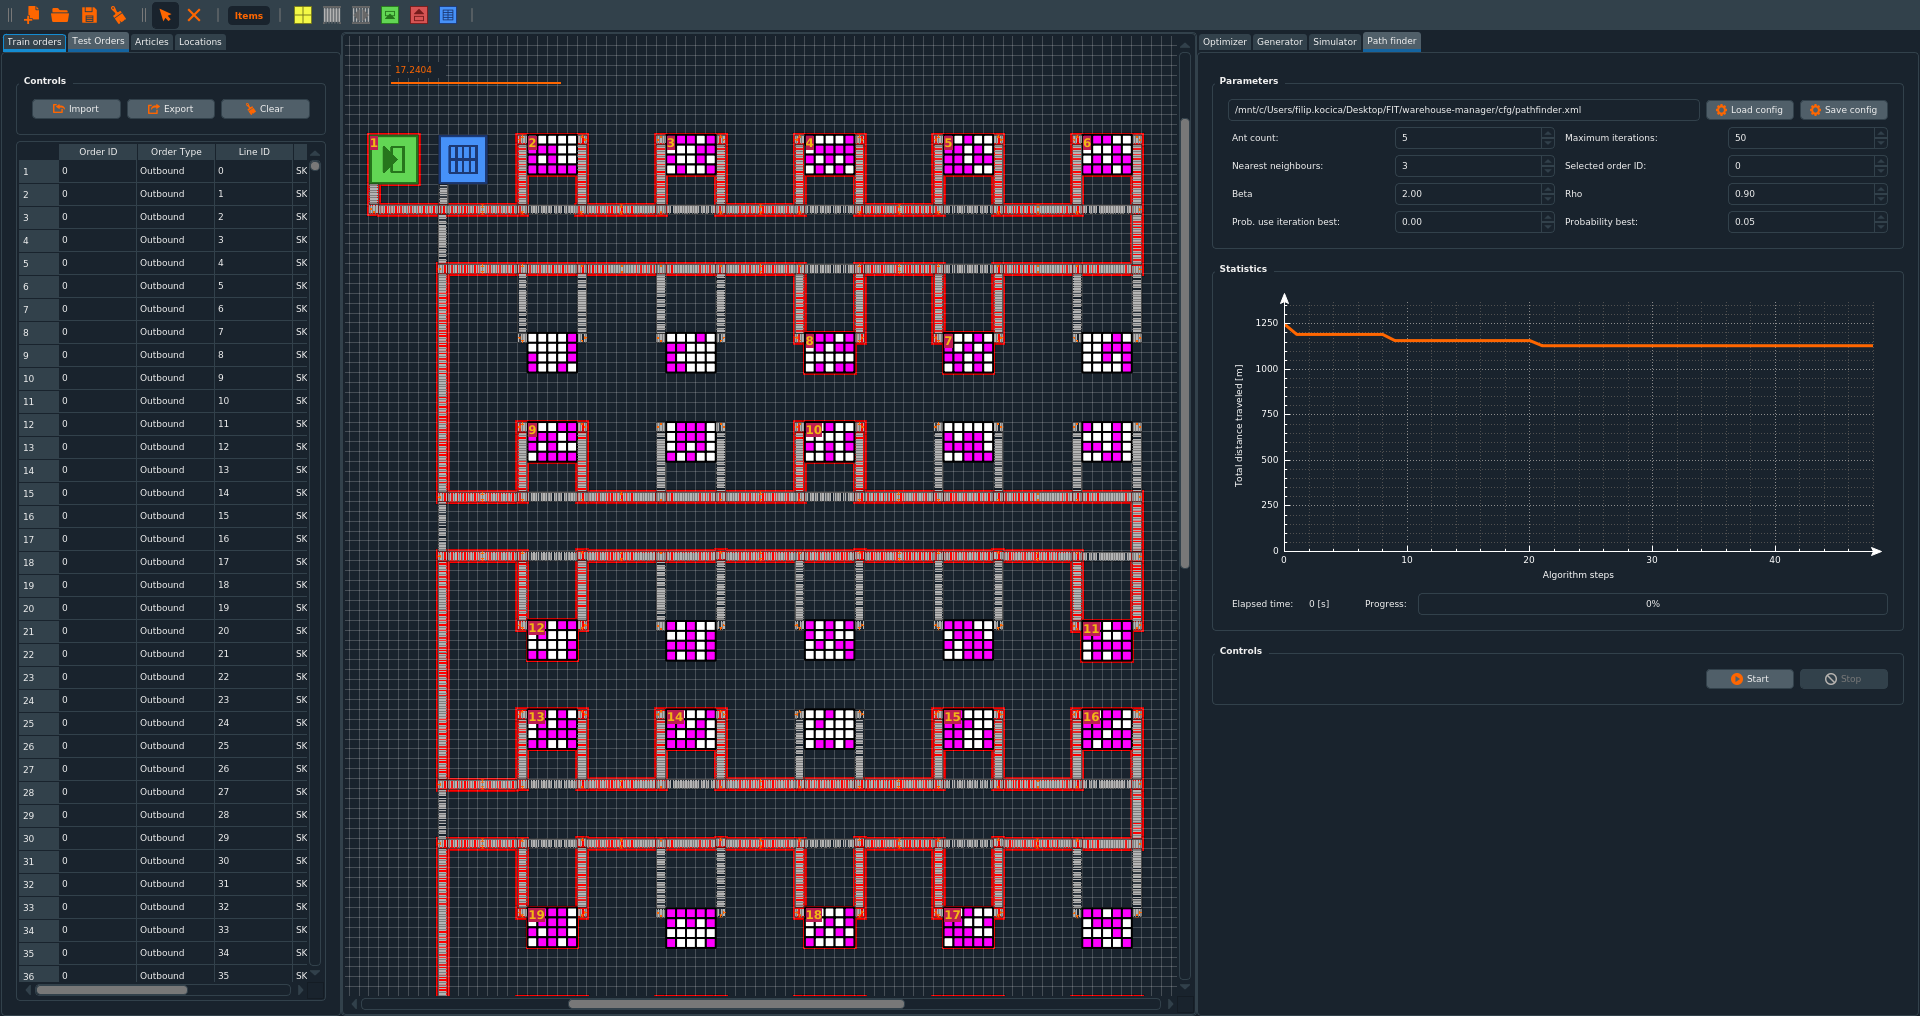
\includegraphics[width=0.99\linewidth]{figures/implementace/WarehouseManagerPaf.png}
    \caption{Grafická implementace nástroje pathfinder zakomponovaná do aplikace Warehouse Manager. Uprostřed je stále plocha pro tvorbu modelu skladu. Vpravo je kontrolní panel, kde je možné nastavit parametry nástroje, sledovat graf objektivní funkce a spustit či zastavit hledání optimální cesty. Vlevo jsou opět data používaná nástrojem (objednávky, produkty a sloty lokací). Nástroj je v grafickém rozhraní implementován v separátním vlákně, aby neblokoval hlavní okno. Po každém kroku optimalizačního algoritmu se však provádí zpětné volání (ang. \emph{callback}) do hlavního vlákna pro přidání nové hodnoty do grafu objektivní funkce a překreslení aktuální nejkratší cesty. Cesta je červeně zvýrazněna a prvky skladu jsou doplněny o čísla aby bylo jasné pořadí, v jakém je bude objednávka navštěvovat.}
    \label{fig:UI_pathFinder}
\end{figure}

\subsection{Princip fungování a implementace}
Na začátku výpočtu se nalezne vstup do skladu (který bude použit vždy jako počátek cesty mravence) a výstup ze skladu (který bude použit vždy jako poslední prvek cesty mravence). Následně se z položek vybrané objednávky zjistí, které lokace musí tato objednávka navštívit (ty budou součástí cesty mezi zmíněným počátkem a koncem). Toto vytvoří graf, který je potřeba projít.

Následně probíhá inicializace matice vzdáleností jednotlivých uzlů (prvků skladu), matice heuristik a nakonec nalezení N (konfigurovatelné) nejbližších sousedů pro každý uzel. Vzdálenost mezi jednotlivými uzly není Eulerova (\uv{vzdušnost čarou}), nýbrž Manhattanská, respektující délku pravoúhle propojených dopravníků propojující tyto dva uzly.

Pro výpočet počátečních limitů hodnot feromonů je nutné sestavit počáteční řešení problému tzv. \uv{hltavým} způsobem, tzn. první jsou do řešení přidáni všichni nejbližší sousedi daného uzlu, a poté zbytek všech uzlů. Poté lze inicializovat matici udávající množství feromonů na přechodech mezi jednotlivými uzly -- kde jsou všechny přechody inicializovány na maximální hodnotu feromonu.

Poté je zahájen výpočet, kdy se v každé iteraci algoritmu sestaví N řešení (mravenců reprezentujících cestu, konfigurovatelné), kterým je následně spočtena délka cesty. Poté je nalezeno nejlepší řešení v dané iteraci a pokud je třeba, tak i aktualizováno dosavadní nejlepší nalezené řešení. Poté je množství feromonu sníženo o míru vypařování a hranám, přes které prochází nejlepší řešení je doplněn feromon v závislosti na kvalitě daného řešení.

Po dosažení před-definovaného množství iterací se vypíše nejlepší nalezený výsledek. V~případě, že je zapnuta i grafická nástavba, jsou průběžné výsledky pomocí zpětného volání posílány do grafického rozhraní (aby se pro každou iteraci mohlo vykreslit nejlepší nalezené řešení) a souběžně je tvořen graf udávající nejkratší délku cesty v každé iteraci, jak lze vidět na snímku \ref{fig:UI_pathFinder}. Tento nástroj je možné použít pro nalezení optimální cesty každé objednávky v simulátoru.

\section{Optimalizátor rozložení produktů}
Automatizované sklady jsou mnohdy velmi komplexní systémy a mají mnohá omezení daná jejich layoutem, způsobem manipulace s produkty, úložnými a pickovacími politikami atd. Optimalizace výkonnosti takovýchto skladů často vyžaduje přesnou definici jejich modelu a nelze jej jednoduše převést na matematický výraz. Vzhledem k tomu, a také k možnosti uživatele si vlastnoručně vytvořit model skladu, by bylo velmi obtížné takto obecně vytvořit matematický popis skladu, proto tato práce pro vyhodnocení kvality používá simulaci, která odpovídá reálnému fungování skladu. Hlavní myšlenka optimalizátoru v této práci je minimalizace doby nutné pro zpracování všech objednávek skrze vhodné rozložení produktů do jednotlivých slotů v lokacích skladu. Doba zpracování objednávek je aproximována simulátorem popsaném v předešlé kapitole. Doba zde představuje simulační čas, nikoli reálný. Grafickou implementaci lze vidět na snímku~\ref{fig:UI_optimalizator}.

Pro nalezení optimální distribuce produktů do slotů lokací byl jako nejvhodnější přístup vybrán GA (genetický algoritmus), a to protože nepotřebuje znát matematický popis problému, pouze problém zakódovat jako sekvenci čísel. Dále byly však pro porovnání implementovány další tři evoluční algoritmy, a sice: DE (diferenční evoluce), ABC (algoritmus umělých včelstev) a PSO (optimalizace rojem částic). Všechny tyto algoritmy pracují standardně ve spojitém prostoru, a tedy bylo potřeba je na základě odborných prací~\cite{ABC_TSP, DE_GA_TSP, PSO_GA_TSP, orderedCrossover, GA_TSP} redefinovat pro diskrétní prostor. K tomu pomohla zejména velká podobnost problematiky SLAP a TSP (problému obchodního cestujícího), pro který byly tyto redefinice v odborných článcích popsány).

\begin{figure}[t]
    \centering
    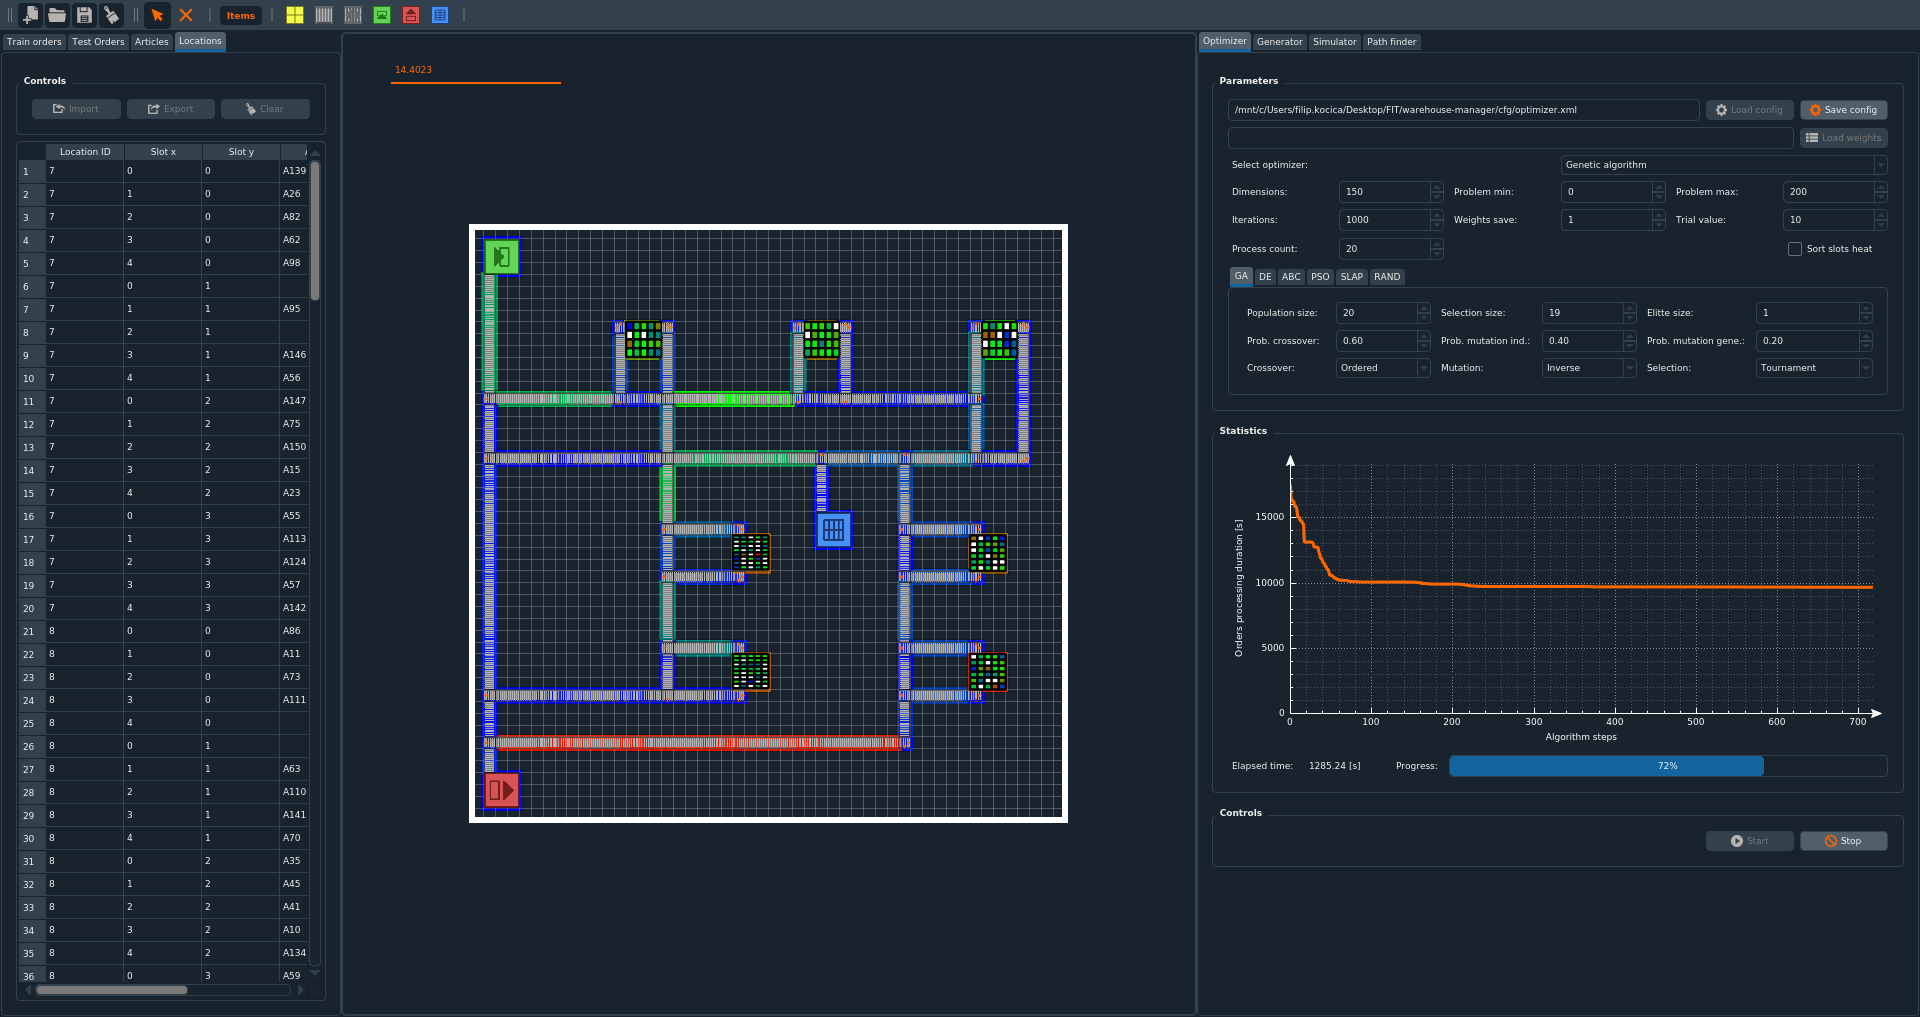
\includegraphics[width=0.99\linewidth]{figures/implementace/WarehouseManagerOpt.png}
    \caption{Grafická implementace optimalizátoru skladu zakomponovaná do aplikace Warehouse Manager. Uprostřed je stále plocha pro tvorbu modelu skladu. Vpravo je kontrolní panel, kde je možné nastavit parametry optimalizace (a vybrat si optimalizační algoritmus a do-nastavit jej v příslušné záložce), vidět graf objektivní funkce a spustit či zastavit optimalizaci. Vlevo jsou opět data používaná optimalizátorem (trénovací objednávky, produkty a sloty lokací). Optimalizátor je v grafickém rozhraní implementován v separátním vlákně, aby neblokoval hlavní okno. Po každém kroku optimalizačního algoritmu se provádí zpětné volání do hlavního vlákna pro přidání nové hodnoty do grafu a překreslení aktuální alokace produktů ve slotech a aktuálního zatížení prvků.}
    \label{fig:UI_optimalizator}
\end{figure}

\subsection{Kódování}
Pro použití evolučních algoritmů bylo nutné navrhnout vhodný způsob kódování řešení. Každý ze čtyř použitých evolučních algoritmů (genetické algoritmy, diferenční evoluce, algoritmus umělých včelstev i optimalizace rojem částic) používají jiné názvosloví. Např. v~genetických algoritmech se pro jedno zakódované řešení problému používá výraz jedinec či chromozom. V algoritmu umělých včelstev je to pak včela či zdroj potravy a v optimalizaci rojem částic je to částice či jedinec. Vzhledem k tomu, že pojem \uv{jedinec} se vyskytuje nejčastěji a nejlépe vystihuje podstatu, bude v tomto textu řešení problému označováno jako jedinec.

\begin{figure}[t]
    \centering
    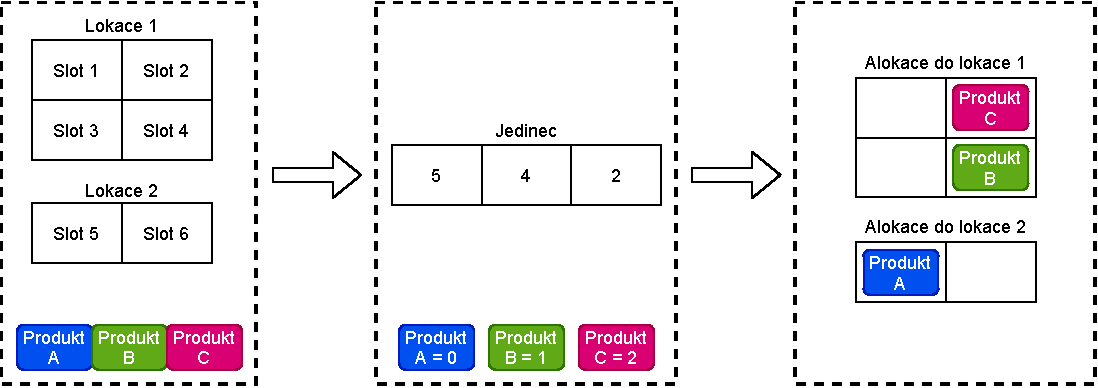
\includegraphics[width=0.99\linewidth]{figures/implementace/ChromosomeEncoding.pdf}
    \caption{Triviální příklad pro navržené kódování. Mějme dvě lokace, první se čtyřmi sloty, druhou se dvěma sloty. Do těchto lokací chceme alokovat tři produkty: A, B, C. Každému slotu je přiřazen unikátní celo-číselný identifikátor. Vezmeme v potaz jednoho jedince populace, který má délku stejnou jako je počet produktů, což je tři. První index reprezentuje první produkt, druhý index druhý produkt atd. Čísla na jednotlivých indexech reprezentují slot, do kterého je produkt alokován. Tzn. produkt A, který obsahuje hodnotu $5$ bude umístěn do slotu $5$, který se nachází v druhé lokaci.}
    \label{fig:chromosomeEncoding}
\end{figure}

Výhodou je, že všechny čtyři algoritmy používají stejné kódování jedinců, proto mohla být vytvořena bázová třída se všemi společnými operacemi (jako inicializace populace, provedení simulace všech jedinců, apod.). Všechny algoritmy byli implementovány ve vlastní třídě vždy odvozené z bázové třídy, což mimo jiné umožnilo využití polymorfismu. Vzhledem k podstatě problému, který byl řešený v diskrétním prostoru, byl zakódovaný jedinec reprezentován jednoduše jako vektor celých čísel. Tento vektor má vždy délku stejnou jako je počet produktů, které se algoritmus snaží optimálně rozdistribuovat do slotů lokací. Jednotlivé položky (zvané jako geny, \emph{allele} hodnoty, apod.) poté nabývají celých čísel reprezentující slot lokace, do kterého bude daný produkt uložen. Všem slotům, které se ve skladu nachází algoritmus přiřadí unikátní celočíselný identifikátor, který se poté používá jako hodnota ve vektoru každého jedince). Příklad znázorňující toto kódování lze najít na obrázku \ref{fig:chromosomeEncoding}.

Tento přístup má však také svá omezení:

\begin{enumerate}
    \item Počet produktů může být rozdílný od počtu slotů lokací, avšak počet slotů musí být vyšší než nebo stejný jako je počet produktů (aby byl každý produkt někam umístěn).
    \item Pokud by bylo provedeno klasické křížení či mutace jedinců bez omezujících podmínek, s velkou pravděpodobností by v jedinci vznikly duplikáty celočíselných hodnot, což by značilo, že více produktů je umístěno do stejného slotu, což není možné.
    \item Bod dva by také implikoval, že některé produkty by nebyly přiřazeny do žádného slotu, což by způsobilo, že objednávky s těmito produkty by nebylo možné dokončit.
\end{enumerate}

Vyjma prvního bodu jsou tyto omezující podmínky v podstatě principiálně stejné, jako tomu je u problému obchodního cestujícího. V podkapitole \ref{section:redefiniceTSP} byla popsána teorie redefinice jednotlivých evolučních algoritmů pro diskrétní prostor a pro řešení problematiky obchodního cestujícího. Tato redefinice byla provedena pro čtyři zmíněné evoluční algoritmy.

\subsection{Grafická teplotní mapa}
Jak lze vidět na snímku \ref{fig:UI_optimalizator}, každý ze zaplněných slotů produktem má jinou barvu. To značí, jak velké má produkt ADU -- tzn. interpretace množství zakoupení produktu pomocí teplotní mapy (ang. \emph{heatmap}). Vzhledem k tomu, že jednotlivé zařízení ve skladu (dopravníky, lokace, ...) mohou mít různé zatížení (t.j. doba, po kterou je zařízení v provozu z~pohledu doby celé simulace), byl implementován mechanismus na zjištění zatížení jednotlivých prvků a jeho grafického znázornění. Grafická vizualizace využívá teplotní mapu na obrázku \ref{fig:heatmap}, a to tak, že kolem jednotlivých prvků vytvoří barevné ohraničení. A tedy nejvíce vytížené prvky budou mít ohraničení rudě červené, zatímco téměř nevyužité prvky tmavě modré. Tento mechanismus by měl uživatelům pomoct identifikovat \uv{úzká místa} ve skladu. Uživatelé pak mohou zkusit přijít na řešení pomocí distribuce zátěže mezi více zařízení a opětovné simulace, nebo nechat optimalizátor se s tímto problémem vypořádat za ně. Přidáním přídavných dopravníků se značně snížila zátěž a průchod skladem se zrychlil. Toto zatížení se v případě textového použití optimalizátoru či simulátoru vypisuje textově.

\addtocounter{footnote}{-1}

\begin{figure}[t]
    \centering
    
\includegraphics[width=0.5\linewidth]{figures/implementace/heatmapOptimizer.png}
    \caption{Grafická vizualizace použité teplotní mapy. Čím jsou produkty častěji kupované (vyšší ADU), tím je barva slotu do kterého jsou umístěny více vpravo (tzn. nejčastěji kupovaný produkt bude reprezentován červeně). Stejná teplotní mapa je použita také pro reprezentaci zatížení skladových prvků jako jsou dopravníky a lokace\protect\footnotemark{}.}
    \label{fig:heatmap}
\end{figure}


\subsection{Konfigurace}
Nástroj lze opět konfigurovat pomocí \texttt{XML} souboru či v grafickém rozhraní a jednotlivé položky které je uživatel schopen nastavit a jejich významy jsou následující -- první blok jsou obecné parametry použité ve více algoritmech, následuje blok s parametry pro genetické algoritmy a zbytek byl pro úsporu místem vynechán:

\begin{itemize}
    \item \texttt{numberDimensions} -- Rozměr problému, neboli velikost jedince.
    \item \texttt{problemMin} -- Nejnižší hodnota, které může gen nabývat.
    \item \texttt{problemMax} -- Nejvyšší hodnota, které může gen nabývat.
    \item \texttt{maxIterations} -- Maximální počet cyklů optimalizačního algoritmu.
    \item \texttt{initialWeights} -- Počáteční váhy (alokace produktů do slotů).
    \item \texttt{saveWeightsPeriod} -- Po kolika cyklech algoritmu se má ukládat nejlepší řešení.
    \item \texttt{maxTrialValue} -- Maximální počet cyklů bez zlepšení fitness, než bude jedinec vyhozen z populace.
    \item \texttt{procCount} -- Počet procesů, které se mají vytvořit pro účely simulace jedinců.
    \item \texttt{slotHeatReorder} -- Produkty v každé z lokací jsou před každým optimalizačním krokem seřazeny podle toho, jak často jsou kupovány.
    \item \texttt{populationSize} -- Velikost populace pro genetické algoritmy.
    \item \texttt{selectionSize} -- Velikost vybrané části pro křížení pro genetické algoritmy.
    \item \texttt{eliteSize} -- Velikost elite (neměnné) části pro genetické algoritmy.
    \item \texttt{probCrossover} -- Pravděpodobnost křížení dvou jedinců.
    \item \texttt{probMutationInd} -- Pravděpodobnost mutace jedince.
    \item \texttt{probMutationGene} -- Pravděpodobnost mutace genu.
    \item \texttt{mutationFunctor} -- Funkce, která se má použít pro mutaci jedince (\texttt{mutateOrdered}, \texttt{mutateInverse}).
    \item \texttt{selectionFunctor} -- Funkce, která se má použít pro selekci jedinců (\texttt{selectRank}, \texttt{selectTrunc}, \texttt{selectTournam}, \texttt{selectRoulette}).
    \item \texttt{crossoverFunctor} -- Funkce, která se má použít pro křížení jedinců (\texttt{crossoverOrdered}, \texttt{crossoverHeuristic}, \texttt{crossoverBinomical}).
    \item A mnoho dalších parametrů pro ABC, DE, PSO, SLAP a náhodné prohledávání\ldots
    %\item \texttt{foodSize} -- Velikost populace (resp. počet včel či zdrojů jídla) algoritmu umělých včelstev.
    %\item \texttt{keepBest} -- Pokud je nastaveno na \uv{pravda}, nejlepší výsledek se nezahazuje (\texttt{trial}).
    %\item \texttt{numberParticles} -- Velikost populace (resp. počet částic) algoritmu optimalizace rojem částic.
    %\item \texttt{correctionFactor1} --  Faktor učení osobní změny.
    %\item \texttt{correctionFactor2} -- Faktor učení sociální změny
    %\item \texttt{weighing} -- Hodnota \emph{inertia}.
    %\item \texttt{crossoverFunctorPSO} -- Funkce, která se má použít pro křížení jedinců (\texttt{crossoverOrdered} viz \ref{fig:orderedCrossover}, \texttt{crossoverHeuristic} viz algoritmus \ref{alg:diskretniPSO}).
    %\item \texttt{populationSizeDE} -- Velikost populace algoritmu diferenční evoluce.
    %\item \texttt{scalingFactor} -- Faktor škálování (reálné číslo, které slouží pro kontrolu rychlosti evoluce).
    %\item \texttt{probCrossoverDE} -- Pravděpodobnost provedení křížení.
    %\item \texttt{crossoverFunctorDE} -- Funkce, která se má použít pro křížení jedinců (\texttt{crossoverOrdered} \ref{fig:orderedCrossover}, \texttt{crossoverBinomical} viz \ref{binomicalCrossover}).
    %\item \texttt{balanceTheLoad} -- Parametr pro SLAP, který pokud je aktivní, tak rozděluje produkty rovnoměrně mezi všechny lokace.
    %\item \texttt{populationSizeRand} -- Velikost \uv{populace} pro náhodné prohledávání.
\end{itemize}

\footnotetext{Obrázek převzat~z~\url{https://stackoverflow.com/a/20793850/8254699}.}


\subsection{Experimenty}
Optimalizace skladu pomocí genetického algoritmu jako taková přinášela velmi dobré výsledky. Avšak stále se nabízely nové způsoby, jak dosáhnout lepších výsledků nebo alespoň podnětného porovnání.

\paragraph{Optimalizátory pro porovnání}
Mimo čtyři optimalizátory rozložení produktů založené na evolučních algoritmech, byly implementovány také dva \uv{optimalizátory} určené čistě pro účely porovnání. První z nich je náhodné prohledávání. Dalším je optimalizátor založený na klasickém přístupu k rozřazení produktů ve skladu převzatý z práce~\cite{slapSeacomp}. Je založený na principu spočtení vzdálenosti každého slotu od vstupního a výstupního bodu skladu, a~jejich seřazení. Dále spočtení, jak často jsou kupovány jednotlivé produkty a jejich seřazení. Následně jsou tyto seřazené produkty namapovány na seřazené sloty lokaci (nejčastěji kupovaný produkt do nejvýhodnějšího slotu, atd.), což by teoreticky mělo vést k~nejvýhodnější alokaci. Porovnání výsledků optimalizace pomocí všech algoritmů na stejném modelu skladu lze vidět na snímku \ref{fig:vyhodnoceniGrafTrain}, ze kterého vyšel jako nejlepší genetický algoritmus, a zmíněný přístup je označen jako \texttt{Batista a spol}.

\paragraph{Třídění produktů v lokacích}
Optimalizace dokázala velmi dobře vyvážit zátěž mezi jednotlivými lokacemi, avšak uskupení produktů ve slotech lokací nebylo úplně ideální. Proto bylo cílem tohoto experimentu řadit produkty ve slotech lokací podle toho, jak často jsou kupovány. To by mělo zrychlit pickování objednávek a ulehčit práci pickerovi. Produkty nejsou přesouvány mezi lokacemi, pouze jsou seřazeny \textbf{v rámci lokace}. Porovnání výsledků lze vidět na snímku \ref{fig:compReordering}. Výsledek při seřazování byl avšak značně horší a tedy se seřazování dále nepoužívalo.

\begin{table}[t]
	\vskip6pt
	\caption{Nejlepší konfigurace genetického algoritmu.}
	\centering
	\begin{tabular}{ll}
		\toprule
		\textbf{Parametr} & \textbf{Hodnota}\\
		\midrule
		Selekce     & Turnaj           \\
		Mutace      & Uspořádaná~\cite{orderedCrossover} \\
		Křížení     & Uspořádané~\cite{orderedCrossover} \\
		Hodnota \emph{trial} & $10$    \\
		Řazení v lokaci      & Vypnuto \\
		Pravděpodobnost křížení         & $0.6$ \\
		Pravděpodobnost mutace jedince  & $0.4$ \\
		Pravděpodobnost mutace genu     & $0.2$ \\
		\bottomrule
	\end{tabular}
	\label{tab:nejConfig}
\end{table}

\paragraph{Kombinování a úprava evolučních algoritmů}
Nejúspěšnější experiment vznikl kombinací algoritmu genetických algoritmů a vlastnosti algoritmu umělých včelstev. Algoritmus umělých včelstev pro každé řešení problému udržuje hodnotu \emph{trial}, která udává počet kroků algoritmu, ve kterých se dané řešení nezlepšilo. Pokud tato hodnota dosáhne před-definované hodnoty, je toto řešení nahrazeno novým náhodně vygenerovaným řešením. Problém u genetických algoritmů byl, že se zasekávaly v lokálních minimech, a proto byly doplněny o tuto vlastnost a poté dosahovaly značně lepších výsledků. Porovnání lze vidět na snímku~\ref{fig:compTrial}.

\begin{figure*}[t]
    \centering
    \begin{minipage}{0.49\textwidth}
        \centering
        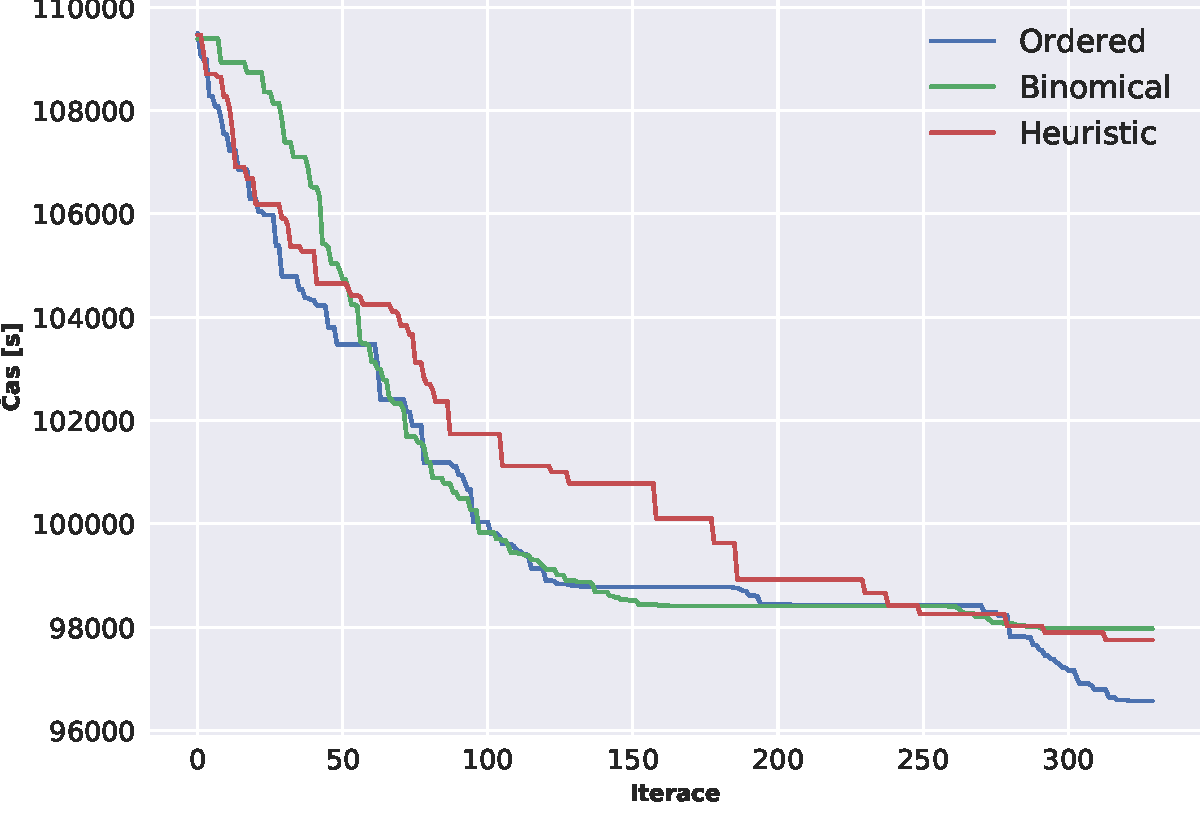
\includegraphics[width=0.99\textwidth]{figures/vyhodnoceni/plotComparisonCrossovers.pdf}
        \caption{Experiment porovnávající různé operátory křížení.}
        \label{fig:compCrossover}
    \end{minipage}\hfill
    \begin{minipage}{0.49\textwidth}
        \centering
        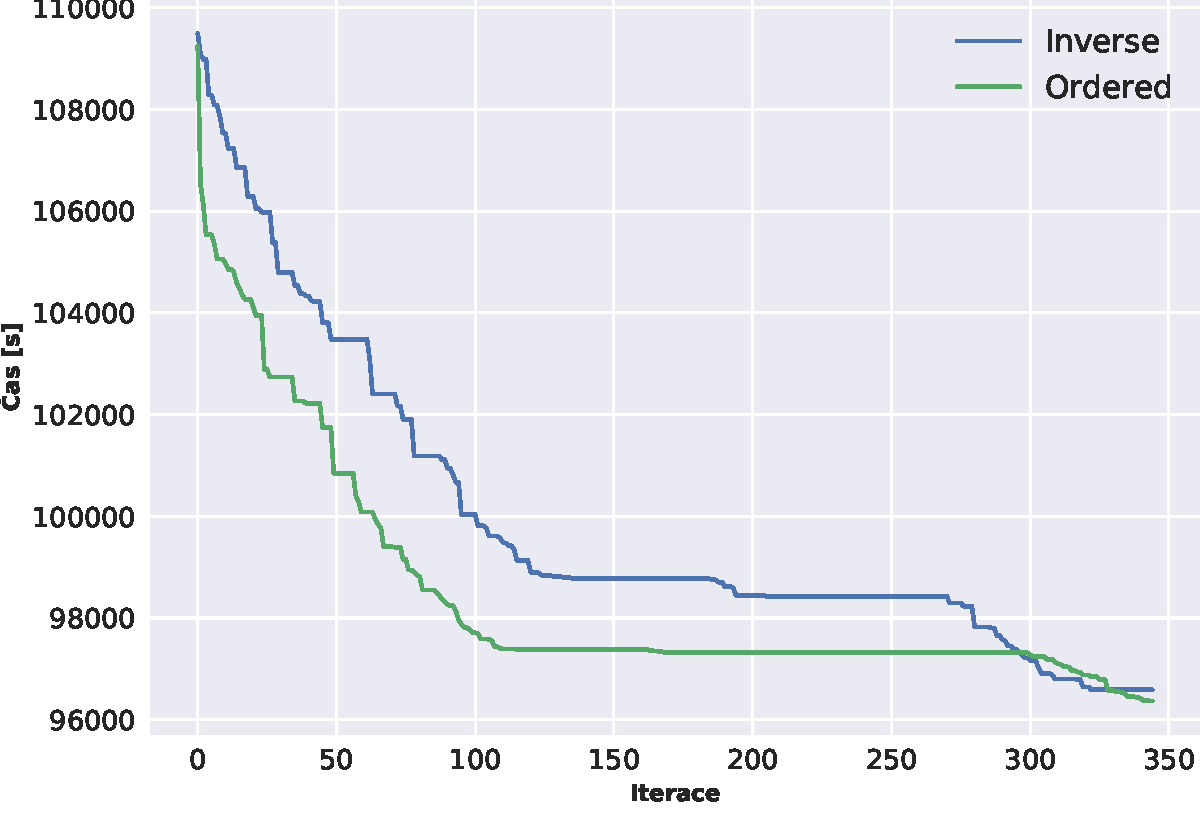
\includegraphics[width=1\textwidth]{figures/vyhodnoceni/plotComparisonMutations.pdf}
        \caption{Experiment porovnávající různé operátory mutace.}
        \label{fig:compMutation}
    \end{minipage}\hfill
\end{figure*}
\begin{figure*}[t]
    \begin{minipage}{0.49\textwidth}
        \centering
        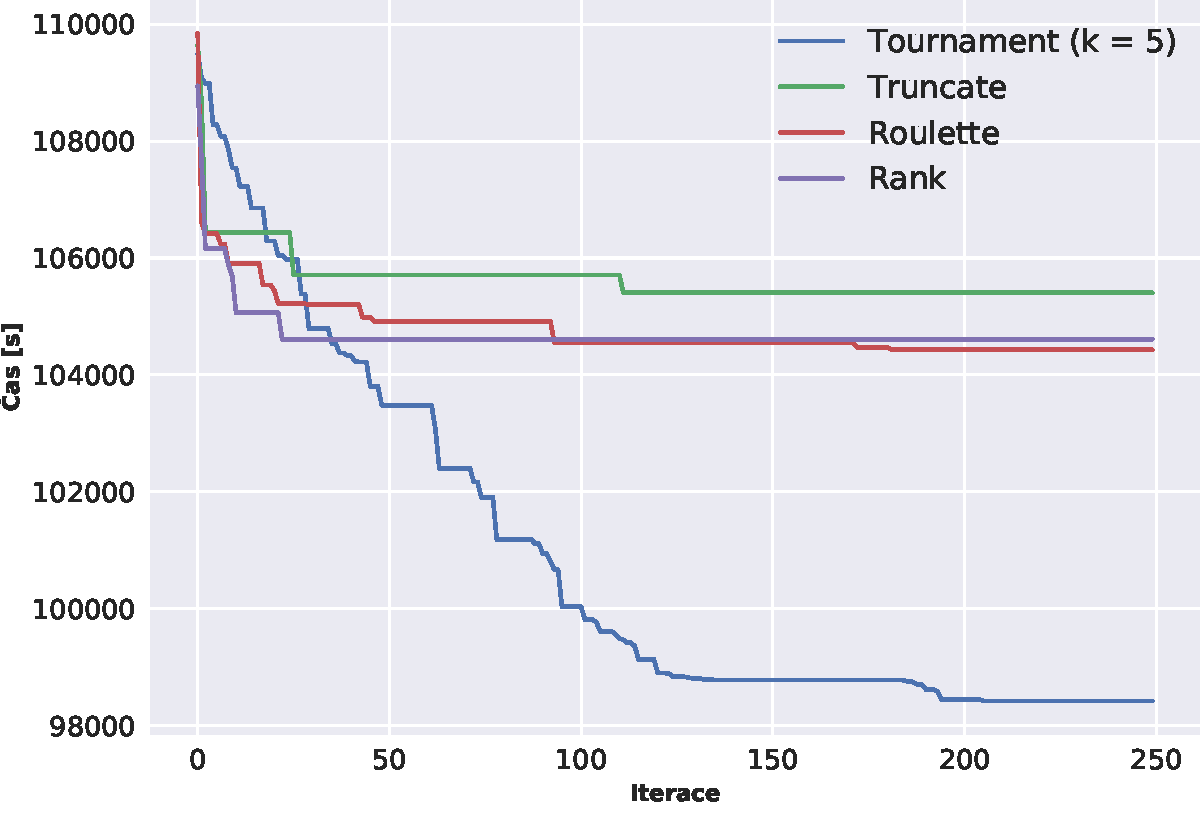
\includegraphics[width=0.99\textwidth]{figures/vyhodnoceni/plotComparisonSelections.pdf}
        \caption{Experiment porovnávající různé operátory selekce.}
        \label{fig:compSelection}
    \end{minipage}\hfill
    \begin{minipage}{0.49\textwidth}
        \centering
        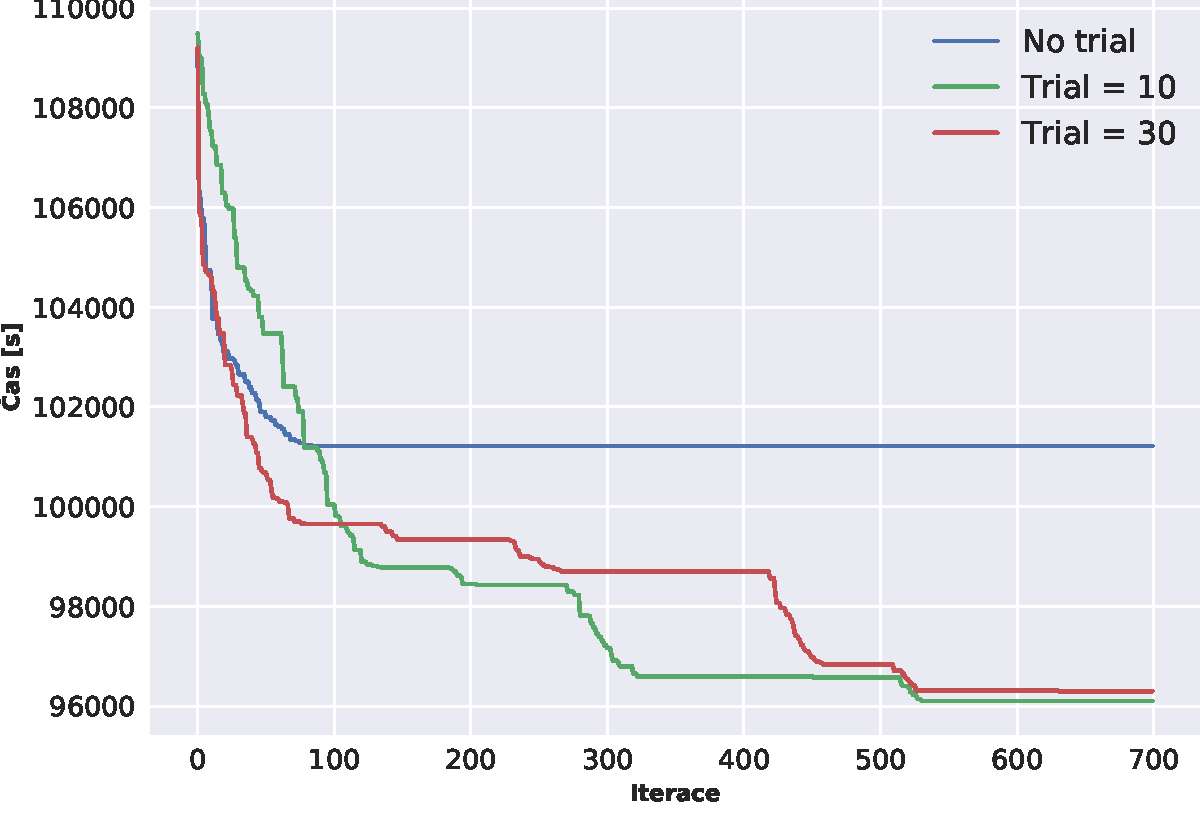
\includegraphics[width=1\textwidth]{figures/vyhodnoceni/plotComparisonTrials.pdf}
        \caption{Experiment porovnávající různé hodnoty $trial$.}
        \label{fig:compTrial}
    \end{minipage}\hfill
\end{figure*}
\begin{figure*}[t]
    \begin{minipage}{0.49\textwidth}
        \centering
        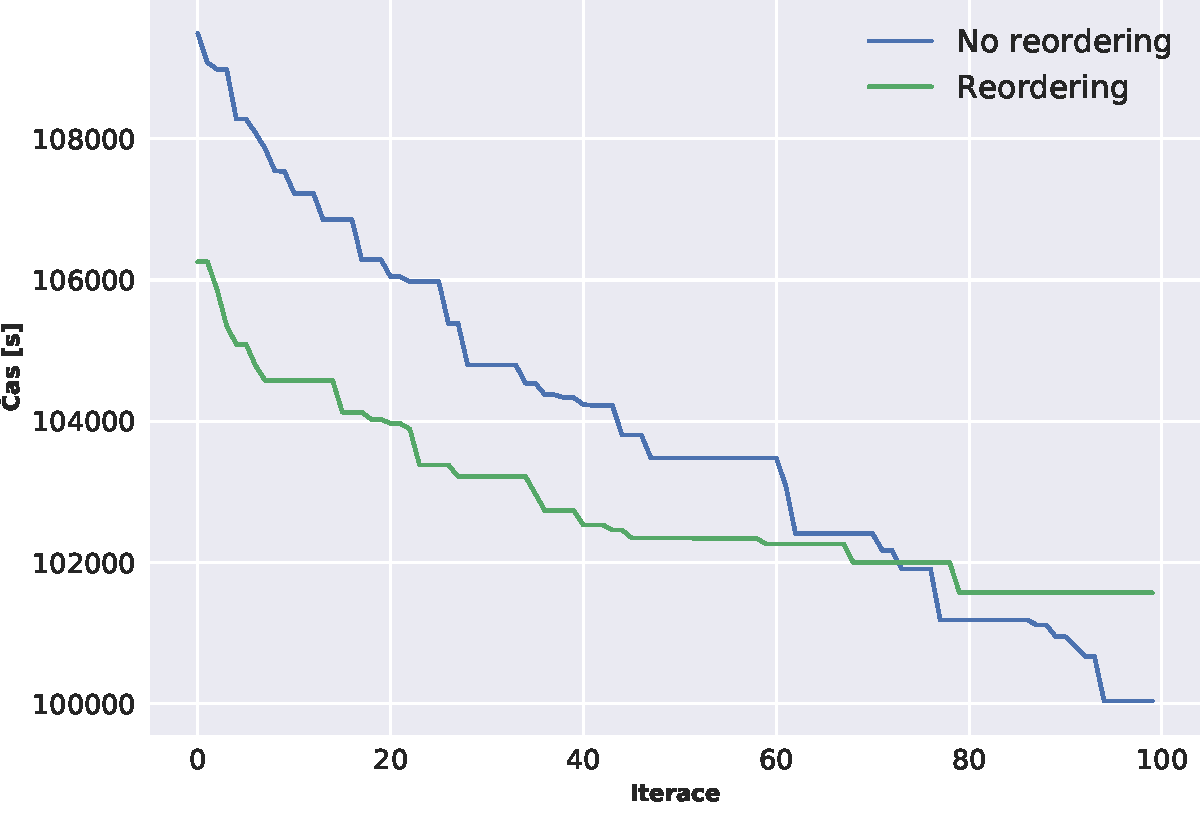
\includegraphics[width=0.99\textwidth]{figures/vyhodnoceni/plotComparisonReordering.pdf}
        \caption{Experiment porovnávající použití uspořádávání a bez použití uspořádávání.}
        \label{fig:compReordering}
    \end{minipage}\hfill
    \begin{minipage}{0.49\textwidth}
        \centering
        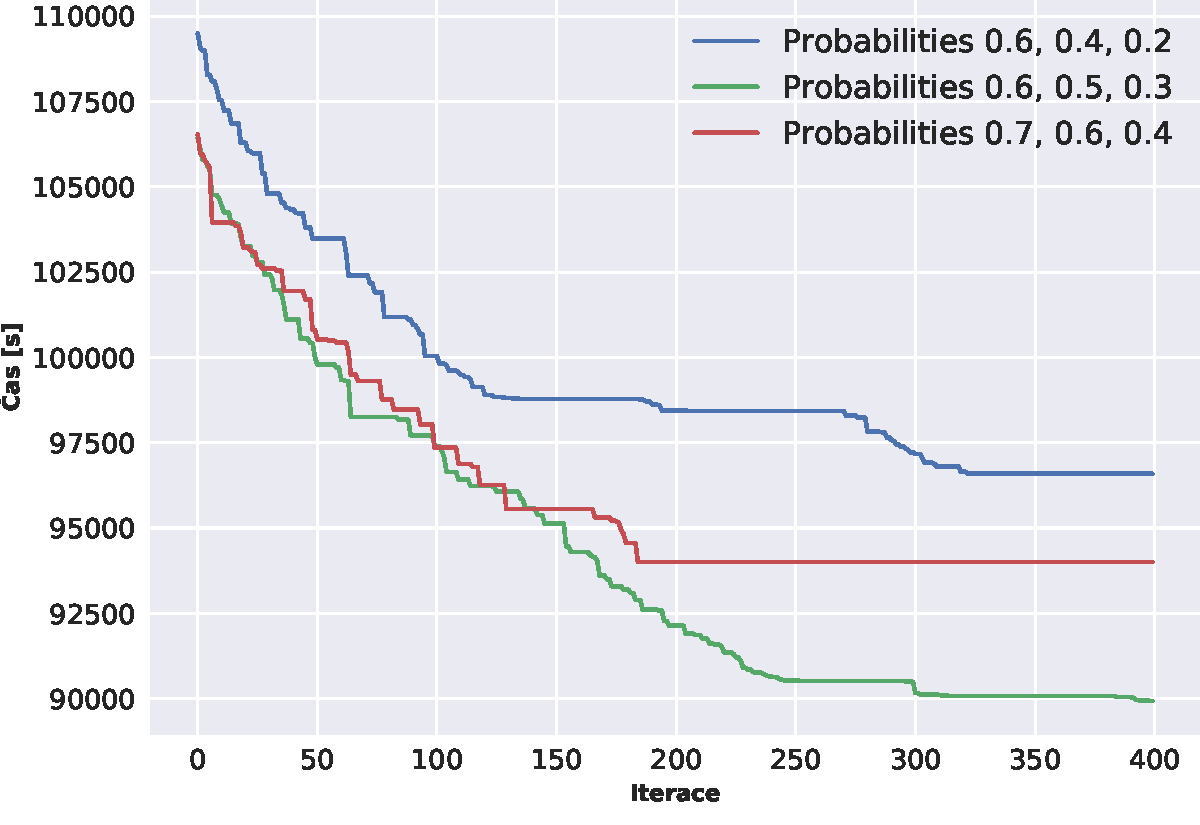
\includegraphics[width=1\textwidth]{figures/vyhodnoceni/plotComparisonParams.pdf}
        \caption{Experiment porovnávající různé pravděpodobnosti provedení křížení a mutace.}
        \label{fig:compParams}
    \end{minipage}\hfill
\end{figure*}

\paragraph{Změna parametrů a vah}
Každý z nástrojů poskytuje bohatou nabídku konfigurací. U~simulátoru je možné například zrychlovat/zpomalovat dopravníky, pracovníky či příchody objednávek. U~těchto hodnot je však vhodné nechat realistickou konfiguraci pro co největší přiblížení izomorfismu s reálným systémem. Optimalizátor umožňuje mimo obecné parametry jako ukládání vah také nastavení různých parametrů evolučních algoritmů. Bylo experimentováno s různými funkcemi pro křížení, mutaci, selekci a dalšími parametry, což značně ovlivňovalo optimalizaci. Pomocí experimentů bylo zjištěno, že nejlepších výsledků dosahuje právě genetický algoritmus a byla nalezena jeho optimální konfigurace, kterou lze najít v tabulce \ref{tab:nejConfig} a v XML souboru přiloženému k aplikaci, aby si jej uživatelé mohli jednoduše načíst. Grafické porovnání lze vidět na snímcích \ref{fig:compCrossover} až \ref{fig:compParams}.

\subsection{Průběh optimalizace}
Ačkoli operace prováděné v evolučních algoritmech jsou zpravidla velmi jednoduchého rázu, v případě této práce velké množství jedinců implikovalo velké množství potřebných simulací a tedy potřebu vysokého výpočetního výkonu pro dosažení rozumné doby optimalizace komplexnějších modelů skladu. Tento problém byl z části řešen tvorbou konfigurovatelného počtu procesů provádějící simulace paralelně~(\ref{section:sim_multithreaded}) a~\uv{eliminací} duplicitních jedinců~(\ref{section:sim_duplicit_jedinci}), avšak stále byla optimalizace na osobním počítači velmi pomalá, nehledě na potřebu neustálého napájení. Z těchto důvodů bylo využito výpočetních zdrojů MetaCentra~\cite{metacentrum}.

MetaCentrum je virtuální organizace poskytující bezplatné výpočetní a úložné kapacity pro členy akademické obce. Uživatelé si mohou na čelním uzlu připravit data a požádat o~naplánování úlohy pomocí PBS (\emph{Portable batch system}). Úlohy lze tvořit buď interaktivní nebo automatizované, ty však vyžadují dávkový soubor. Po přidělení požadovaných prostředků (s většími nároky na zdroje roste i doba než jsou prostředky přiděleny) je úloha spuštěna na jednom z výpočetních uzlů. Požádat o výpočetní zdroje a spuštění úlohy definované dávkovým souborem lze následujícím způsobem:
$$\texttt{qsub -l select=1:ncpus=64:mem=1gb:scratch\_local=1gb:walltime=24:00:00 ga.sh}$$
Tento příkaz do fronty vloží požadavek na 64 procesorů, 1GB paměti RAM, 1GB prostoru na disku a dobu alokace těchto prostředků na 24 hodin. Po přidělení prostředků je proveden obsah dávkového souboru \texttt{ga.sh} na výpočetním uzlu -- to zpravidla zahrnovalo nakopírování zdrojových kódů aplikace \emph{Warehouse Manager} na výpočetní uzel, sestavení programu, použití požadovaného konfiguračního souboru a začátek trénování. V konfiguračním souboru bylo možné nastavit počáteční váhy modelu, a nezačínat tak trénování vždy od znovu. V průběhu výpočtu se průběžně podle konfigurace ukládaly váhy (aby nebyly ztraceny dosažené výsledky v případě pádu aplikace) a po dokončení úlohy nakopírování těchto dosažených výsledků zpět na úložiště.

\section{Warehouse Manager}
Grafická aplikace, ve výsledku nazvaná Warehouse Manager disponuje mimo původní účel (t.j. tvorba 2D modelu skladu), také veškerými funkcionalitami implementovanými v rámci této práce. To znamená veškerou kontrolu nad simulátorem, generátorem, pathfinderem i~optimalizátorem. To umožňuje možnost plného využití této práce i technicky méně zdatným jedincům, jako např. logistickým manažerům, zcela bez nutnosti využít příkazovou řádku.

\subsection{Layout aplikace}
Rozložení grafické aplikace bylo vytvořeno za pomoci aplikace \texttt{Qt Designer}: v horní liště lze najít tlačítka pro ovládání, jako např. vytvoření nového modelu skladu, načtení již existujícího modelu ze souboru, atd. Dále se v této liště nachází jednotlivé prvky/zařízení skladu, které může uživatel využít pro vytvoření modelu skladu. Na levé straně aplikace jsou záložky, které slouží pro import, export a náhled dat využívaných jednotlivými nástroji, jako jsou (zleva): objednávky pro trénování a testování, produkty a lokace se sloty, které mohou obsahovat i aktuální alokaci produktů do daných slotů. Vpravo jsou opět záložky, které slouží pro přepínání mezi jednotlivými nástroji. Každý z těchto čtyř nástrojů má ve své záložce následující části:

\begin{itemize}
    \item \textbf{Konfigurace} -- Zde jsou veškeré parametry, které daný nástroj poskytuje a lze je předvyplnit konfiguračním souborem, či je exportovat do XML.
    \item \textbf{Statistiky} -- Zde jsou obsaženy grafy, do kterých jsou postupně doplňovány hodnoty produkované daným nástrojem.
    \item \textbf{Řízení} -- Poskytuje tlačítka pro kontrolu jednotlivých nástrojů, jako je spuštění či zastavení. Ve chvíli, kdy je spuštěn jeden z uvedených nástrojů, jsou veškerá kontrolní tlačítka, stejně tak úprava modelu skladu, zakázána. A to aby uživatel nijak nenarušil běh daného nástroje. Naopak se povolí tlačítko pro zastavení běhu nástroje. Zastavení nebo dokončení práce nástrojem opět povolí úpravu modelu skladu a veškerá tlačítka.
\end{itemize}

Uprostřed aplikace je plocha určená pro tvorbu a manipulaci s modelem skladu. Cílem této plochy je poskytnout úplný a intuitivní 2D editor poskytující různé druhy skladových prvků a manipulaci s nimi. Ve výsledku editor (mimo jiné) umožňuje:

\begin{itemize}
    \item Měřítko vůči reálnému světu.
    \item Změnu velikosti, pozice a rotaci prvků.
    \item Propojování skladových prvků pomocí portů.
    \item Hromadnou selekci a kopírování prvků.
    \item Zobrazení podrobných informací o prvku.
    \item Uložení modelu skladu do souboru a načtení ze souboru.
    \item Přiblížení a oddálení scény/modelu skladu\footnote{Inspirováno \url{https://stackoverflow.com/a/19114517/8254699}.}.
\end{itemize}

\subsection{Tvorba modelu skladu}
\label{sec:uiModelSkladu}
Uživatel, který chce aplikaci plně využít ve svůj prospěch, musí být schopen vytvořit model skladu dle jeho potřeb. Zejména pro tyto účely byla grafická aplikace navržena, a později doplněna o veškerou ostatní funkcionalitu. Pro implementaci plochy pro tvorbu modelu skladu byla využita grafická scéna (\texttt{QGraphicsScene}\footnote{\url{https://doc.qt.io/qt-5/qgraphicsscene.html}}) a grafický pohled (\texttt{QGraphicsView}\footnote{\url{https://doc.qt.io/qt-5/qgraphicsview.html}}). Do grafické scény jsou postupně umisťovány prvky skladu odvozené od grafických prvků (\texttt{QGraphicsItem}\footnote{\url{https://doc.qt.io/qt-5/qgraphicsitem.html}}), doplňující je o specifickou funkcionalitu. Při implementaci byly využity volně dostupné doplňky \texttt{Qt}: \texttt{QDarkStyleSheet}\footnote{\url{https://github.com/ColinDuquesnoy/QDarkStyleSheet}}, \texttt{QCustomPlot}\footnote{\url{https://www.qcustomplot.com}} a \texttt{QtEditableItems}\footnote{\url{https://github.com/fadyosman/QtEditableItems}}.

\subsubsection{Grafická scéna}
Grafický pohled umožňuje zobrazení grafické scény ve widgetu. Grafická scéna slouží jako kontejner grafických prvků a v kombinaci s grafickým pohledem slouží k vizualizaci takovýchto prvků na 2D povrchu. Pro účely přepsání jistých vlastností grafické scény (jako např. zobrazení kontextového menu) byla tato třída odvozena. Stejně tak grafické prvky, které byly do scény umisťovány, byly odvozeny a velmi značně přepsány pro daný \emph{use-case}. Takovéto odvození umožnilo například vytvoření manipulátorů pro změnu velikosti prvků a také jejich rotaci, viz \ref{fig:uiItemInfo}. Uživatel je na začátku práce dotázán na velikost skladu v metrech. Tyto rozměry jsou interně přepočteny a je vytvořeno ohraničení skladu bílými čarami, mřížkou pro jednodušší manipulaci s prvky a také měřítkem (vlevo nahoře). Délka měřítka je vždy jedna pětina šířky grafické scény, a číslo nad ní udává, kolik metrů ve skutečnosti tato délka (část scény) reprezentuje.

Grafický pohled a scéna byly doplněny mimo jiné také o možnost přibližování a oddalování, bez kterých by byla aplikace jen velmi těžce použitelná. Tohoto lze dosáhnout pomocí přidržení klávesy \texttt{CTRL} a pohybem rolovacího tlačítka myši. Při této akci se také přepočítává měřítko vůči reálnému světu. Pro usnadnění tvorby komplexních modelů skladu byla implementována možnost hromadného označování prvků a následně možnost kopírování a~přemisťování označených prvků, což může velmi usnadnit tvorbu modelu.

\subsubsection{Grafické prvky}
Jak již bylo zmíněno, grafické prvky jsou odvozeny z \texttt{QGraphicsItem}. Poté jsou z této odvozené třídy odvozeny další třídy pro každý typ zařízení, a sice:

\begin{itemize}
    \item \texttt{UiWarehouseItemLocation\_t} -- Reprezentuje lokace.
    \item \texttt{UiWarehouseItemConveyor\_t} -- Reprezentuje dopravníky.
    \item \texttt{UiWarehouseItemGate\_t} -- Reprezentuje vstupní a výstupní brány skladu.
\end{itemize}

Veškeré grafické prvky jsou reprezentovány jako ukazatele na dynamicky alokovanou paměť, tzv. \uv{hromadu} (ang. \emph{heap}), a to z důvodu aby grafické prvky existovaly i po opuštění rozsahu části programu, kde jsou vytvořeny. O uvolnění paměti se poté starají mechanismy frameworku Qt díky specifikaci rodičovských prvků, až po hlavní okno. Tzn. při destrukci rodiče jsou uvolněni veškeří následníci, poté jejich následníci, a tak dále. Jednotlivé třídy jsou rozšířeny o funkcionalitu specifickou pro dané zařízení skladu. Např. lokace je rozšířena o mřížku slotů, tedy kontejner instancí třídy \texttt{UiWarehouseSlot\_t} atd.

Propojování grafických prvků lze provádět na základě portů -- \texttt{UiWarehousePort\_t} (oranžové šipky na každém z prvků, viz \ref{fig:uiItemInfo}). Po připojení daného portu k jinému se tyto spojené porty skryjí a ukáží se opět při odpojení prvku. Každé ze zařízení má jiný počet portů, dle jeho způsobu použití.

\begin{figure}[t]
    \centering
    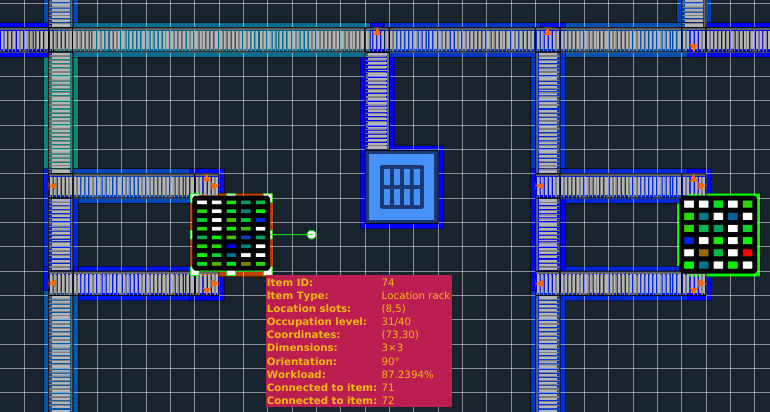
\includegraphics[width=0.95\linewidth]{figures/implementace/UI_model_info.png}
    \caption{Zobrazení informací o zařízení skladu pomocí najetí kurzorem (přesně se jedná o lokaci). Dále lze na snímku vidět porty sloužící k propojování prvků (oranžové šipky) a nakonec také manipulátory, pomocí kterých lze vybraný prvek rotovat a měnit jeho velikost.}
    \label{fig:uiItemInfo}
\end{figure}


Informace o~grafickém prvku lze zobrazit pomocí najetí myší na daný prvek, viz \ref{fig:uiItemInfo}. V~zobrazené tabulce lze najít veškeré informace o~prvku, ať už jde o~pozici, velikost a~natočení, nebo specifické informace jako zatížení prvku nebo úroveň obsazenosti lokace.

\subsubsection{Serializace modelu skladu}
Model skladu může být poměrně komplexní, a~jeho opětovné vytváření při každém spuštění by nedávalo smysl. Proto je možné model serializovat (uložit) do souboru ve formátu XML (pomocí knihovny \texttt{libxml2}), a také jej ze souboru deserializovat (načíst) do grafického rozhraní. Velmi jednoduchý příklad lze vidět na následujícím výpisu.
\newpage
\lstset{
    language=xml,
    tabsize=3,
    %frame=lines,
    caption=Test,
    label=code:sample,
    frame=shadowbox,
    rulesepcolor=\color{gray},
    xleftmargin=20pt,
    framexleftmargin=15pt,
    keywordstyle=\color{blue}\bf,
    commentstyle=\color{OliveGreen},
    stringstyle=\color{red},
    numbers=left,
    numberstyle=\tiny,
    numbersep=5pt,
    breaklines=true,
    showstringspaces=false,
    basicstyle=\footnotesize,
    emph={food,name,price},emphstyle={\color{magenta}}}
    \lstinputlisting[caption={Serializovaný model skladu ve formátu XML. První element obsahuje informace o layoutu, jako je výška, šířka a kolik jeden metr představuje bodů ve scéně. Další element představuje dopravník i s informacemi, kde se ve scéně nachází, jak je velký a jak je natočený. Následuje lokace, která mimo pozici apod. obsahuje také informaci o slotech. Následuje jediný propoj vytvořený mezi těmito dvěma prvky.}]{data/layout.xml}

    
\section{Moduly programu}
V této sekci jsou velmi krátce popsány jednotlivé moduly programu, které jsou v různé míře využity všemi implementovanými nástroji. Operátor rozsahu platnosti zde identifikuje jednotlivé jmenné prostory, ve kterých jsou moduly uloženy:

\begin{itemize}
    \item \texttt{whm::ConfigParser\_t} -- Tento modul slouží pro serializaci a de-serializaci konfiguračních souborů v XML, a umožňuje získávání konfiguračních hodnot pomocí šablonové metody.
    \item \texttt{whm::Logger\_t} -- Komplexní modul pro zaznamenávání běhu aplikace na výstup či do souboru.
    \item \texttt{whm::utils::*} -- Utility (šablonové funkce) plošně využívané v celé aplikaci.
    \item \texttt{whm::WarehouseDataGenerator\_t} -- Modul který obstarává generování zákaznických objednávek.
    \item \texttt{whm::WarehouseSimulatorSIMLIB\_t} -- Modul který obstarává simulaci skladu pomocí knihovny \texttt{SIMLIB/C++}.
    \item \texttt{whm::WarehousePathFinder\_t} -- Modul, který rekurzivně vyhledá veškeré cesty ve skladu, uloží do vhodné datové struktury a umožňuje nalezení nejkratší cesty mezi lokacemi, apod.
    \item \texttt{whm::WarehousePathFinderACO\_t} -- Implementace mravenčího algoritmu pro nalezení nejkratší cesty objednávky skrze celý sklad.
    \item \texttt{whm::WarehouseOptimizer\{Base|GA|DE|ABC|PSO|SLAP|RAND\}\_t} -- Implementace\newline čtyř evolučních algoritmů v diskrétním prostoru, metodiky SLAP, náhodného prohledávání a bázové třídy, ze které jsou všechny optimalizátory odvozeny. Optimalizátory využívají definici řešení problému definovaného v modulu \texttt{whm::Solution\_t}.
    \item \texttt{whm::WarehouseOrder\_t} -- Modul implementující zákaznickou objednávku.
    \item \texttt{whm::WarehouseOrderLine\_t} -- Modul implementující část (položku) zákaznické objednávky.
    \item \texttt{whm::WarehouseLocationRack\_t} -- Modul implementující lokaci, která se skládá ze slotů a jsou v ní uloženy produkty.
    \item \texttt{whm::WarehouseLocationSlot\_t} -- Modul implementující sloty, ze kterých sestává lokace.
    \item \texttt{whm::WarehousePort\_t} -- Modul implementující port pomocí kterého lze propojovat jednotlivé prvky.
    \item \texttt{whm::WarehouseConnection\_t} -- Modul implementující propojení prvků ve skladu.
    \item \texttt{whm::WarehouseItem\_t} -- Modul implementující prvek/zařízení skladu.
    \item \texttt{whm::WarehouseLayout\_t} -- Modul poskytující \emph{singleton}, který obsahuje veškeré důležité informace o celém skladu.
    \item \texttt{whm::gui::*} -- Grafická nástavba textového klienta (souborů výše), která sestává z~cca. 15 modulů, mimo jiné také z vláken, které složí k provádění náročných operací jako je např. optimalizace -- aby neblokovaly hlavní smyčku (grafické okno). Dále pak z odvozených grafických prvků, scény, apod. Pokud je definován symbol \texttt{WHM\_GUI}, jsou některé moduly v seznamu nahoře doplněny o zpětné volání do grafického rozhraní. 
\end{itemize}
